\section{Hai đường thẳng vuông góc}
\subsection{Góc giữa hai đường thẳng trong không gian}
\begin{dn}
	\immini
	{
		\textbf{Góc giữa hai đường thẳng} $a$, $b$ trong không gian, kí hiệu $(a,b)$, là góc giữa hai đường thẳng $a'$ và $b'$ cùng đi qua một điểm và lần lượt song song hoặc trùng với $a$ và $b$.
	}
	{
		\begin{tikzpicture}[scale=0.8,font=\footnotesize]
			\def \c{0.5}
			\def \d{-0.7}
			\coordinate[label=above:$O$] (O) at (0,0);
			\fill (O)circle(1.5pt);
			\path
			(-2,-2*\c) coordinate (A1)
			(3,3*\c) coordinate (B1)
			(-0.2,-0.2*\c+1) coordinate (A2)
			(2.5,2.5*\c+1) coordinate (B2)
			(-2,-2*\d) coordinate (C1)
			(2,2*\d) coordinate (D1)
			(-0.4,-0.4*\d-0.8) coordinate (C2)
			(1.8,1.8*\d-0.8) coordinate (D2)
			($(O)!0.8!(B1)$)node[above]{$a$}
			($(O)!0.5!(D1)$)node[above]{$b$}
			($(A2)!0.3!(B2)$)node[above]{$a'$}
			($(C2)!0.7!(D2)$)node[above]{$b'$}
			;
			\draw (A1)--(B1)
			(A2)--(B2)
			(C1)--(D1)
			(C2)--(D2)
			;
		\end{tikzpicture}
	}
\end{dn}
\begin{note}
	\begin{enumerate}[a)]
		\item Để xác định góc giữa hai đường thẳng $a$, $b$ ta có thể lấy một điểm $O$ nằm trên một trong hai đường thẳng đó và vẽ đường thẳng song song với đường thẳng còn lại.
		\item Góc giữa hai đường thẳng nhận giá trị từ $0^{\circ}$ đến $90^{\circ}$.
	\end{enumerate}
\end{note}
\subsection{Hai đường thẳng vuông góc trong không gian}
\begin{dn}
	Hai đường thẳng $a$, $b$ được gọi là vuông góc với nhau nếu góc giữa chúng bằng $90^{\circ}$.
\end{dn}
Hai đường thẳng $a$, $b$ vuông góc được kí hiệu là $a\perp b$ hoặc $b\perp a$.
\begin{note}
	\begin{enumerate}
		\item Hai đường thẳng vuông góc có thể cắt nhau hoặc chéo nhau.
		\item Cho hai đường thẳng song song, đường thẳng nào vuông góc với đường này thì cũng vuông góc với đường kia.
		\item Trong không gian, khi có hai đường thẳng phân biệt $a$, $b$ cùng vuông góc với một đường thẳng thứ ba $c$ thì ta chưa kết luận được $a\parallel b$ như trong hình học phẳng.
	\end{enumerate}
\end{note}

\begin{dang}{Xác định góc giữa hai đường thẳng trong không gian}
	\immini{
		\begin{itemize}
			\item Muốn xác định góc giữa hai đường thẳng $a$ và $b$, ta dời song song hai đường thẳng $a$, $b$ về $a'$, $b'$ chung gốc rồi tính góc.
			\begin{itemize}
				\item Ta có $\heva{&a\parallel a'\\&b\parallel b'}\Rightarrow(a,b)=\left(a',b'\right)$.
				\item Nếu $a\parallel b$ hoặc $a\equiv b$ thì $(a,b)=0^{\circ}$.
			\end{itemize}
			\item Nhắc lại định lý cosin trong tam giác $ABC$
			\begin{itemize}
				\item $\cos{\widehat{BAC}}=\dfrac{AB^{2}+AC^{2}-BC^{2}}{2\cdot AB\cdot AC}$.
				\item $\cos{\widehat{ABC}}=\dfrac{AB^{2}+BC^{2}-AC^{2}}{2\cdot AB\cdot BC}$.
				\item $\cos{\widehat{BCA}}=\dfrac{BC^{2}+AC^{2}-AB^{2}}{2\cdot BC\cdot AC}$.
			\end{itemize}
		\end{itemize}
	}{
		\begin{tikzpicture}[scale=0.8,font=\footnotesize]
			\def \c{0.5}
			\def \d{-0.7}
			\coordinate[label=above:$O$] (O) at (0,0);
			\fill (O)circle(1.5pt);
			\path
			(-2,-2*\c) coordinate (A1)
			(3,3*\c) coordinate (B1)
			(-0.2,-0.2*\c+1) coordinate (A2)
			(2.5,2.5*\c+1) coordinate (B2)
			
			(-2,-2*\d) coordinate (C1)
			(2,2*\d) coordinate (D1)
			(-0.4,-0.4*\d-0.8) coordinate (C2)
			(1.8,1.8*\d-0.8) coordinate (D2)
			
			($(O)!0.8!(B1)$)node[above]{$a'$}
			($(O)!0.5!(D1)$)node[above]{$b'$}
			($(A2)!0.3!(B2)$)node[above]{$a$}
			($(C2)!0.7!(D2)$)node[above]{$b$}
			;
			\draw (A1)--(B1)
			(A2)--(B2)
			(C1)--(D1)
			(C2)--(D2)
			;
		\end{tikzpicture}
	}
\end{dang}
\begin{note}
	\begin{itemize}
		\item Để xác định góc giữa hai đường thẳng chéo nhau $a$ và $b$, ta có thể lấy một điểm $O$ thuộc đường thẳng $a$ và qua đó kẻ đường thẳng $b'$ song song với $b$. Khi đó $(a,b)=\left(a,b'\right)$.
		\item Với hai đường thẳng $a$, $b$ bất kì ta có $0^{\circ}\leq(a,b)\leq 90^{\circ}$.
		\item Nếu $a$ song song hoặc trùng với $a'$ và $b$ song song hoặc trùng với $b'$ thì $(a,b)=\left(a',b'\right)$.
	\end{itemize}
\end{note}
%%%=============VD_1=============%%%
\begin{vd}%[1H8H1-3]%[Dự án đề cương 3 Khối NH 24-25- Dot 2 - Nguyễn Trần Anh Tuấn]
	Cho hình hộp $ABCD.A'B'C'D'$ có $6$ mặt đều là hình vuông và $M$, $N$, $E$, $F$ lần lượt là trung điểm các cạnh $BC$, $BA$, $AA'$, $A'D'$. Tính góc giữa các cặp đường thẳng
	\begin{multicols}{2}
		\begin{enumerate}
			\item $A'C'$ và $BC$;
			\item $MN$ và $EF$.
		\end{enumerate}
	\end{multicols}
	\loigiai{
		\immini{
			\begin{enumerate}
				\item Ta có $AC\parallel A'C'$.\\
				Suy ra $\left(A'C',BC\right)=(AC,BC)=\widehat{ACB}=45^{\circ}$\\
				(vì $\triangle ACB$ vuông cân tại $B$).
				\item Ta có $\heva{&AC\parallel MN\\&AD'\parallel EF.}$\\
				Suy ra $(MN,EF)=\left(AC,AD'\right)=\widehat{CAD'}=60^{\circ}$\\ (vì $\triangle ACD'$ đều).
			\end{enumerate}
		}{
			\begin{tikzpicture}[declare function={r=3;},font=\scriptsize]
				\path (0:0) coordinate (A)
				(0:r) coordinate (B)
				++(37:{0.65*r}) coordinate (C)
				++(180:r) coordinate (D)
				\foreach \x in {A,B,C,D}{(\x)++(90:r) coordinate (\x_1)}
				($(B)!0.5!(C)$) coordinate (M)
				($(B)!0.5!(A)$) coordinate (N)
				($(A_1)!0.5!(A)$) coordinate (E)
				($(A_1)!0.5!(D_1)$) coordinate (F);
				\draw[dashed] (D_1)--(D)--(A) (D)--(C) (A)--(C) (M)--(N) (E)--(F) (A)--(D_1)--(C);
				\draw (A)--(B)--(C) (A)--(A_1) (B)--(B_1) (C)--(C_1)(A_1)--(B_1)--(C_1)--(D_1)--cycle (A_1)--(C_1);
				\foreach \x/\goc/\t in {A/255/A, B/-75/B, C/10/C, D/170/D, A_1/135/A', B_1/90/B',
					C_1/45/C', D_1/90/D',M/0/M,N/-90/N,E/180/E,F/90/F}{
					\draw[fill=white] (\x) circle (1pt) node[shift={(\goc:9pt)}]{$\t$};
				}
			\end{tikzpicture}
		}
		
	}
\end{vd}
%%%=============================%%%

%%%=============VD_2=============%%%
\begin{vd}%[1H8H1-3]%[Dự án đề cương 3 Khối NH 24-25- Dot 2 - Nguyễn Trần Anh Tuấn]
	Cho hình chóp $S.ABCD$ có đáy là hình thoi cạnh $a$, $SA=a\sqrt 3$, $SA\perp BC$. Tính góc giữa hai đường thẳng $SD$ và $BC$.
	\loigiai{
		\immini{Ta có
			$\heva{&SA\perp BC\\&BC\parallel AD}\Rightarrow SA\perp AD$.\\ Do đó
			$(SD,BC)=(SD,AD)=\widehat{SDA}$.\\
			Xét $\triangle SAD$ vuông tại $A$ ta có
			\begin{eqnarray*}
				&&\tan SDA=\dfrac{SA}{DA}=\dfrac{a\sqrt3}{a}=\sqrt{3}\\
				&\Rightarrow&\widehat{SDA}=60^{\circ}.
			\end{eqnarray*}
			Vậy góc giữa hai đường thẳng $SD$ và $BC$ bằng $60^{\circ}$.
		}
		{
			\begin{tikzpicture}[declare function={gocx=90; goc=-150; a=3; b=a/2; h=3;}]
				\path (0,0) coordinate (A)--+(gocx:h) coordinate (S)
				(a,0) coordinate (B)
				(goc:b) coordinate (D)
				+(a,0) coordinate (C);
				\draw pic[angle radius=2mm,draw] {right angle = S--A--B};
				\draw[dashed] (S)--(A) (D)--(A)--(B);
				\draw (S)--(D)--(C)--(S)--(B)--(C)--cycle;
				\foreach \x/\goc in {S/90,A/150,B/0,C/-60,D/-180}
				\draw[fill=white] (\x) node[shift={(\goc:7pt)},font=\scriptsize]{$\x$} circle (1pt);
		\end{tikzpicture}}
	}
\end{vd}
%%%=============================%%%

%%%=============VD_3=============%%%
\begin{vd}%[1H8H1-3]%[Dự án đề cương 3 Khối NH 24-25- Dot 2 - Nguyễn Trần Anh Tuấn]
	Cho tứ diện $ABCD$. Gọi $M$, $N$ lần lượt là trung điểm của $BC$, $AD$. Biết $AB=CD=a$ và $MN=\dfrac{a\sqrt{3}}{2}$. Tính góc giữa hai đường thẳng $AB$ và $CD$.
	\loigiai{
		\immini{
			Gọi $P$ là trung điểm của $BD$.\\
			Ta có $\heva{&NP\parallel AB\\&MP\parallel CD}\Rightarrow(AB,CD)=(NP,MP)$.\\
			Xét $\triangle MNP$ ta có
			$MP=NP=\dfrac{a}{2}$ và
			\begin{eqnarray*}
				&&\cos \widehat{MPN}=\dfrac{MP^{2}+NP^{2}- MN^{2}}{2MP\cdot NP}=-\dfrac{1}{2}\\
				&\Rightarrow& \widehat{MPN}
				= 120^{\circ}\\
				&\Rightarrow&(MP,NP)=60^{\circ}.
			\end{eqnarray*}
			Vậy góc giữa hai đường thẳng $AB$ và $CD$ là $60^{\circ}$.
		}{
			\begin{tikzpicture}[declare function={goc=-60; a=5; b=0.45*a; h=5;}]
				\path
				(0,0) coordinate (A)
				(a,0) coordinate (C)
				(goc:b) coordinate (B)--+(0,h) coordinate (D)
				($(C)!0.5!(B)$) coordinate (M)
				($(A)!0.5!(D)$) coordinate (N)
				($(B)!0.5!(D)$) coordinate (P);
				\draw[dashed] (A)--(C) (M)--(N);
				\draw (D)--(B) (D)--(A)--(B)--(C)--cycle (M)--(P)--(N);
				\foreach \x/\goc in {D/90,A/240,C/-60,B/-90,M/-90,N/180,P/180}
				\draw[fill=white] (\x) node[shift={(\goc:7pt)},font=\scriptsize]{$\x$} circle (1pt);
			\end{tikzpicture}
		}
	}
\end{vd}
%%%=============================%%%
\begin{dang}{Chứng minh hai đường thẳng vuông góc trong không gian}
	\begin{itemize}
		\item \textbf{Cách 1:} Nếu góc giữa hai đường thẳng bằng $90^{\circ}$ thì ta kết luận hai đường thẳng vuông góc.\\
		\item \textbf{Cách 2:} Sử dụng liên hệ giữa quan hệ song song và vuông góc $\heva{& a\parallel b\\&c\perp a}\Rightarrow c\perp b $.
	\end{itemize}
\end{dang}
%%%=============VD_1=============%%%
\begin{vd}%[1H8H1-3]%[Dự án đề cương 3 Khối NH 24-25- Dot 2 - Nguyễn Trần Anh Tuấn]
	Cho hình hộp $ABCD.A'B'C'D'$ có $6$ mặt đều là hình vuông. Chứng minh rằng
	\begin{multicols}{2}
		\begin{enumerate}
			\item $AB\perp CC'$.
			\item $AC\perp B'D'$.
		\end{enumerate}
	\end{multicols}
	\loigiai{
		\immini{
			\begin{enumerate}
				\item Ta có $CC'\parallel BB'$.\\
				Suy ra $\left(AB, CC'\right)=\left(AB, BB'\right)=\widehat{ABB'}=90^{\circ}$.\\ Vậy $AB\perp CC'$.
				\item Ta có $B'D'\parallel BD$.\\Suy ra $\left(AC, B'D'\right)=(AC, BD)=90^{\circ}$ (hai đường chéo của hình vuông luôn vuông góc với nhau).\\ Vậy $AC\perp B'D'$.
			\end{enumerate}
		}
		{
			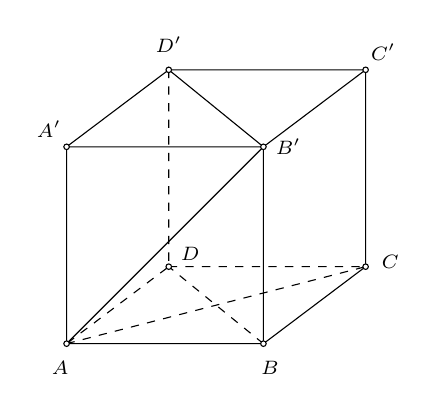
\begin{tikzpicture}[declare function={r=2.5;},font=\scriptsize]
				\path (0:0) coordinate (A)
				(0:r) coordinate (B)
				++(37:{0.65*r}) coordinate (C)
				++(180:r) coordinate (D)
				\foreach \x in {A,B,C,D}{(\x)++(90:r) coordinate (\x_1)};
				\draw[dashed] (D_1)--(D)--(A) (D)--(C) (A)--(C) (B)--(D);
				\draw (A)--(B)--(C) (A)--(A_1) (B)--(B_1) (C)--(C_1)(A_1)--(B_1)--(C_1)--(D_1)--cycle (A)--(B_1) (B_1)--(D_1);
				\foreach \x/\goc/\t in {A/255/A, B/-75/B, C/10/C, D/30/D, A_1/135/A', B_1/0/B',
					C_1/45/C', D_1/90/D'}{
					\draw[fill=white] (\x) circle (1pt) node[shift={(\goc:9pt)}]{$\t$};
				}
			\end{tikzpicture}
		}
	}
\end{vd}
%%%=============================%%%

%%%=============VD_2=============%%%
\begin{vd}%[1H8H1-3]%[Dự án đề cương 3 Khối NH 24-25- Dot 2 - Nguyễn Trần Anh Tuấn]
	Cho hình chóp $S.ABC$ có $SA=SB=SC=a$, $\widehat{BSA}=\widehat{CSA}=60^{\circ}$, $\widehat{BSC}=90^{\circ}$. Cho $I$ và $J$ lần lượt là trung điểm của $SA$ và $BC$. Chứng minh rằng $IJ\perp SA$ và $IJ\perp BC$.
	\loigiai{
		\immini{
			Ta có $\triangle SAB$ và $\triangle SAC$ cân tại $S$.\\
			Lại có $\widehat{BSA}=\widehat{CSA}=60^{\circ}$.\\
			Khi đó $\triangle SAB$ và $\triangle SAC$ là các tam giác đều.\\ Suy ra $AB=AC=a$.\\
			Ta có $\triangle SBC$ vuông cân tại $S$ suy ra $BC=SB\sqrt{2}=a\sqrt{2}$.\\
			Khi đó $\triangle BAC$ vuông cân tại $A$ (định lý Pytago đảo).\\
			$\triangle SBC$ và $\triangle ABC$ là các tam giác vuông cân có cùng cạnh huyền $BC$, $J$ là trung điểm của $BC\Rightarrow JS=JA\left(=\dfrac{BC}{2}\right)$.\\
			$\triangle JSA$ cân tại $J$ có $JI$ là đường trung tuyến suy ra $JI\perp SA$.\\
			Ta thấy $IB$ và $IC$ là các đường cao của tam giác đều có cùng cạnh $a$, suy ra $IB=IC$. \\
			$\triangle IBC$ cân tại $I$ có $IJ$ là đường trung tuyến nên $IJ\perp BC$.
		}{
			\begin{tikzpicture}[declare function={goc=-65; a=5; b=0.45*a; h=5;}]
				\path
				(0,0) coordinate (A)
				(a,0) coordinate (C)
				(goc:b) coordinate (B)
				($(C)!.5!(B)$) coordinate (J)
				($(A)!.66!(J)$) coordinate (H)
				+(0,h) coordinate (S)
				($(A)!0.5!(S)$) coordinate (I);
				\foreach \x/\y/\z in {B/A/C,B/S/C}{
					\path (\y) pic[draw,angle radius=5pt]{right angle = \x--\y--\z};
				}
				\draw[dashed] (J)--(A)--(C) (J)--(I) (C)--(I);
				\draw (S)--(B) (S)--(A)--(B)--(C)--cycle (S)--(J) (B)--(I);
				\foreach \x/\goc in {S/90,A/240,C/-60,B/-90,J/-40,I/180}
				\draw[fill=white] (\x) node[shift={(\goc:7pt)},font=\scriptsize]{$\x$} circle (1pt);
			\end{tikzpicture}
		}
	}
\end{vd}
%%%=============================%%%

%%%=============VD_3=============%%%
\begin{vd}%[1H8H1-3]%[Dự án đề cương 3 Khối NH 24-25- Dot 2 - Nguyễn Trần Anh Tuấn]
	Cho hình chóp $S.ABCD$ có đáy là hình vuông $ABCD$ cạnh bằng $a$ và các cạnh bên đều bằng $a$. Gọi $M$ và $N$ lần lượt là trung điểm của $AD$ và $SD$. Chứng minh $MN\perp SC$.
	\loigiai{
		\immini{
			Ta có
			$MN\parallel SA\Rightarrow\left(MN,SC\right)=\left(SA,SC\right)$.\\
			$AC=a\sqrt{2}\Rightarrow AC^{2}=SA^{2}+SC^{2}$.\\
			$\Rightarrow\triangle SAC$ vuông tại $S$ (định lý Pythagore đảo).\\
			Suy ra $\widehat{ASC}=90^{\circ}$ hay $\left(MN,SC\right)=\left(SA,SC\right)=90^{\circ}$.\\
			Vậy $MN\perp SC$.
		}
		{
			\begin{tikzpicture}[declare function={goc=-150; a=4; b=a/2; h=a;}]
				\path (0,0) coordinate (A)
				(a,0) coordinate (B)
				(goc:b) coordinate (D)
				+(a,0) coordinate (C)
				($(A)!.5!(C)$) coordinate (O)--+(0,h) coordinate (S)
				($(S)!0.5!(D)$) coordinate (N)
				($(A)!0.5!(D)$) coordinate (M);
				\draw pic[angle radius=3mm,draw] {right angle = S--O--D};
				\draw pic[angle radius=3mm,draw] {right angle = B--A--D};
				\draw[dashed] (S)--(A) (D)--(A)--(B) (S)--(O) (A)--(C) (D)--(B) (M)--(N);
				\draw (S)--(D)--(C)--(S)--(B)--(C)--cycle;
				\foreach \x/\goc in {S/90,A/150,B/0,C/-60,D/-180,O/-90,M/-10,N/150}
				\draw[fill=white] (\x) node[shift={(\goc:7pt)},font=\scriptsize]{$\x$} circle (1pt);
			\end{tikzpicture}
		}
	}
\end{vd}
%%%=============================%%%

\subsection{Bài tập rèn luyện}
\ind{PHẦN I.} \inden{Câu trắc nghiệm nhiều phương án lựa chọn. Mỗi câu hỏi học sinh chỉ chọn một phương án.}\\
\setcounter{ex}{0}
\Opensolutionfile{ans}[ans/1H8-Bai1-TN]
%%%=============EX_1=============%%%
\begin{ex}[Trích đề thi HKII - THPT Chuyên Lê Quý Đôn, Ninh Thuận - Năm học: 2024-2025]%[1H8N1-3]%[Dự án đề cương 3 Khối NH 24-25- Dot 2 - Nguyễn Trần Anh Tuấn]
	Cho hình chóp $S.ABCD$ có đáy là hình chữ nhật, cạnh $SA$ vuông góc với đáy. Góc giữa hai đường thẳng $BC$ và $SD$ bằng
	\choice
	{$\widehat{SBC}$}
	{$\widehat{SAC}$}
	{\True $\widehat{SDA}$}
	{$\widehat{SAD}$}
	\loigiai{
		\immini{
			Vì $BC\parallel AD$ nên $\left(BC,SD\right)=\left(AD,SD\right)=\widehat{SDA}$ (vì $\widehat{SDA}$ là góc nhọn).}
		{
			\begin{tikzpicture}[declare function={gocx=90; goc=-150; a=3; b=a/2; h=3;}]
				\path (0,0) coordinate (A)--+(gocx:h) coordinate (S)
				(a,0) coordinate (B)
				(goc:b) coordinate (D)
				+(a,0) coordinate (C);
				\draw pic[angle radius=3mm,draw] {right angle = S--A--B};
				\draw[dashed] (S)--(A) (D)--(A)--(B);
				\draw (S)--(D)--(C)--(S)--(B)--(C)--cycle;
				\foreach \x/\goc in {S/90,A/150,B/0,C/-60,D/-180}
				\draw[fill=white] (\x) node[shift={(\goc:7pt)},font=\scriptsize]{$\x$} circle (1pt);
			\end{tikzpicture}
		}
	}
\end{ex}
%%%=============================%%%

%%%=============EX_2=============%%%
\begin{ex}%[1H8N1-3]%[Dự án đề cương 3 Khối NH 24-25- Dot 2 - Nguyễn Trần Anh Tuấn]
	Cho hình lập phương $ABCD.EFGH$. Góc giữa hai đường thẳng $EH$ và $BD$ là
	\choice
	{\True $45^{\circ}$}
	{$90^{\circ}$}
	{$60^{\circ}$}
	{$120^{\circ}$}
	\loigiai{
		\immini{
			Ta có
			$EH\parallel AD$.\\
			Suy ra $\left(EH,BD\right)=\left(AD,BD\right)=\widehat{ADB}=45^{\circ}$.\\
			Vậy góc giữa hai đường thẳng $EH$ và $BD$ bằng $45^{\circ}$.
		}
		{
			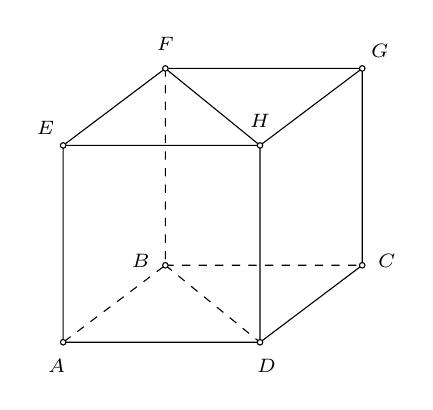
\begin{tikzpicture}[declare function={r=2.5;},font=\scriptsize]
				\path (0:0) coordinate (A)
				(0:r) coordinate (B)
				++(37:{0.65*r}) coordinate (C)
				++(180:r) coordinate (D)
				\foreach \x in {A,B,C,D}{(\x)++(90:r) coordinate (\x_1)};
				\draw[dashed] (D_1)--(D)--(A) (D)--(C) (D)--(B);
				\draw (A)--(B)--(C) (A)--(A_1) (B)--(B_1) (C)--(C_1)(A_1)--(B_1)--(C_1)--(D_1)--cycle (D_1)--(B_1);
				\foreach \x/\goc/\t in {A/255/A, B/-75/D, C/10/C, D/170/B, A_1/135/E, B_1/90/H,
					C_1/45/G, D_1/90/F}{
					\draw[fill=white] (\x) circle (1pt) node[shift={(\goc:9pt)}]{$\t$};
				}
			\end{tikzpicture}
		}
	}
\end{ex}
%%%=============================%%%

%%%=============EX_3=============%%%
\begin{ex}%[1H8N1-3]%[Dự án đề cương 3 Khối NH 24-25- Dot 2 - Nguyễn Trần Anh Tuấn]
	Cho hình lập phương $ABCD.EFGH$. Góc giữa hai đường thẳng $FH$ và $ED$ là
	\choice
	{$45^{\circ}$}
	{\True $60^{\circ}$}
	{$90^{\circ}$}
	{$120^{\circ}$}
	\loigiai{
		\immini{
			Ta có
			$FH\parallel BD$.\\
			Suy ra $\left(FH,ED\right)=\left(BD,ED\right)=\widehat{BDE}=60^{\circ}$ (do $\triangle EBD$ đều). \\
			Vậy góc giữa $FH$ và $ED$ bằng $60^{\circ}$.
		}
		{
			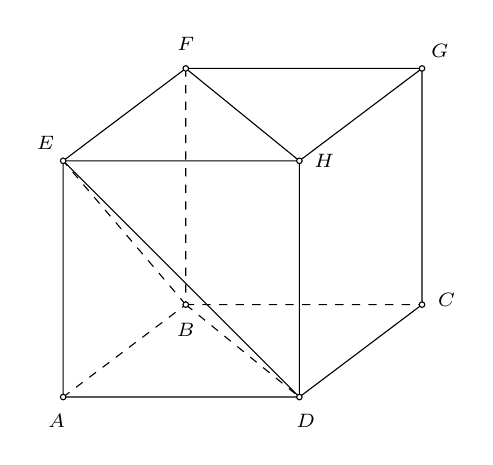
\begin{tikzpicture}[declare function={r=3;},font=\scriptsize]
				\path (0:0) coordinate (A)
				(0:r) coordinate (B)
				++(37:{0.65*r}) coordinate (C)
				++(180:r) coordinate (D)
				\foreach \x in {A,B,C,D}{(\x)++(90:r) coordinate (\x_1)};
				\draw[dashed] (D_1)--(D)--(A) (D)--(C) (D)--(B) (D)--(A_1);
				\draw (A)--(B)--(C) (A)--(A_1) (B)--(B_1) (C)--(C_1)(A_1)--(B_1)--(C_1)--(D_1)--cycle (D_1)--(B_1) (B)--(A_1);
				\foreach \x/\goc/\t in {A/255/A, B/-75/D, C/10/C, D/-90/B, A_1/135/E, B_1/0/H,
					C_1/45/G, D_1/90/F}{
					\draw[fill=white] (\x) circle (1pt) node[shift={(\goc:9pt)}]{$\t$};
				}
			\end{tikzpicture}
		}
	}
\end{ex}
%%%=============================%%%

%%%=============EX_4=============%%%
\begin{ex}[Trích đề thi GHKII - THPT Lương Thế Vinh - Đồng Nai - Năm học: 2024-2025]%[1H8N1-3]%[Dự án đề cương 3 Khối NH 24-25- Dot 2 - Nguyễn Trần Anh Tuấn]
	Cho tứ diện đều $ABCD$ cạnh $a$. Góc giữa $AB$ và $BC$ bằng
	\choice
	{\True $60^{\circ}$}
	{$90^{\circ}$}
	{$30^{\circ}$}
	{$120^{\circ}$}
	\loigiai{
		\immini{
			Ta có $(AB,BC)=\widehat{ABC}=60^{\circ}$ (vì $\triangle ABC$ đều).
		}
		{
			\begin{tikzpicture}[declare function={r=2;}]
				\path (90:{r*1.25}) coordinate (A)
				(160:{r} and {r*0.35}) coordinate (B)
				(20:{r} and {r*0.35}) coordinate (C)
				(260:{r} and {r*0.5}) coordinate (D);
				\draw[dashed] (B)--(C);
				\draw (A)--(D) (A)--(B)--(D)--(C)--cycle;
				\foreach \x/\goc in {A/90,B/120,C/60,D/-90}
				\draw[fill=white] (\x) node[shift={(\goc:7pt)},font=\scriptsize]{$\x$} circle (1pt);
			\end{tikzpicture}
		}
	}
\end{ex}
%%%=============================%%%

%%%=============EX_5=============%%%
\begin{ex}%[1H8N1-1]%[Dự án đề cương 3 Khối NH 24-25- Dot 2 - Nguyễn Trần Anh Tuấn]
	Góc giữa hai đường thẳng trong không gian là
	\choice
	{\True Góc giữa hai đường thẳng cùng đi qua một điểm và lần lượt song song với hai đường thẳng đã cho}
	{Góc giữa hai đường thẳng cùng đi qua một điểm và song song với một trong hai đường thẳng đã cho}
	{Góc giữa hai đường thẳng song song với một trong hai đường thẳng đã cho}
	{Góc giữa hai đường thẳng cùng đi qua một điểm}
	\loigiai{
		Định nghĩa góc giữa hai đường thẳng.
	}
\end{ex}
%%%=============================%%%

%%%=============EX_6=============%%%
\begin{ex}%[1H8N1-1]%[Dự án đề cương 3 Khối NH 24-25- Dot 2 - Nguyễn Trần Anh Tuấn]
	Trong không gian, mệnh đề nào sau đây là đúng?
	\choice
	{\True Một đường thẳng vuông góc với một trong hai đường thẳng song song thì vuông góc với đường thẳng còn lại}
	{Hai đường thẳng cùng vuông góc với một đường thẳng thì vuông góc với nhau}
	{Hai đường thẳng cùng vuông góc với một đường thẳng thì song song với nhau}
	{Một đường thẳng vuông góc với một trong hai đường thẳng vuông góc thì song song với đường thẳng còn lại}
	\loigiai{\lq\lq Một đường thẳng vuông góc với một trong hai đường thẳng song song thì vuông góc với đường thẳng còn lại\rq\rq~là mệnh đề đúng.
	}
\end{ex}
%%%=============================%%%

%%%=============EX_7=============%%%
\begin{ex}%[1H8N1-1]%[Dự án đề cương 3 Khối NH 24-25- Dot 2 - Nguyễn Trần Anh Tuấn]
	Hai đường thẳng được gọi là vuông góc với nhau nếu góc giữa chúng có số đo
	\choice
	{nhỏ hơn $90^{\circ}$}
	{\True bằng $90^{\circ}$}
	{lớn hơn $90^{\circ}$}
	{từ $0^{\circ}$ đến $90^{\circ}$}
	\loigiai{
		Hai đường thẳng được gọi là vuông góc với nhau nếu góc giữa chúng có số đo bằng $90^{\circ}$.
	}
\end{ex}
%%%=============================%%%

%%%=============EX_8=============%%%
\begin{ex}[Trích đề thi giữa HKII THPT Edison - Hải Phòng- Năm học: 2024-2025]%[1H8N1-1]%[Dự án đề cương 3 Khối NH 24-25- Dot 2 - Nguyễn Trần Anh Tuấn]
	Góc giữa hai đường thẳng bất kì trong không gian là góc giữa
	\choice
	{Hai đường thẳng lần lượt vuông góc với nhau}
	{Hai đường thẳng cắt nhau và lần lượt vuông góc với nhau}
	{\True Hai đường thẳng cùng đi qua một điểm và lần lượt song song với chúng}
	{Hai đường thẳng cắt nhau và không song song với nhau}
	\loigiai{
		Theo định nghĩa: \lq\lq Góc giữa hai đường thẳng $m$ và $n$ trong không gian, kí hiệu $(m, n)$, là góc giữa hai đường thẳng $a$ và $b$ cùng đi qua một điểm và tương ứng song song với $m$ và $n$\rq\rq.
	}
\end{ex}
%%%=============================%%%

%%%=============EX_9=============%%%
\begin{ex}%[1H8H1-2]%[Dự án đề cương 3 Khối NH 24-25- Dot 2 - Nguyễn Trần Anh Tuấn]
	Cho hình lập phương $ABCD.A'B'C'D'$. Đường thẳng nào sau đây vuông góc với đường thẳng $BC'$?
	\choice
	{\True $A'D$}
	{$AC$}
	{$BB'$}
	{$AD'$}
	\loigiai{
		\immini{Ta có $\heva{&A'D\parallel B'C\\&B'C\perp BC'}\Rightarrow A'D\perp BC'$.
		}
		{
			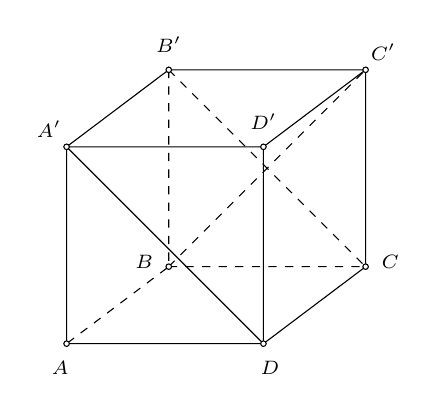
\begin{tikzpicture}[declare function={r=2.5;},font=\scriptsize]
				\path (0:0) coordinate (A)
				(0:r) coordinate (B)
				++(37:{0.65*r}) coordinate (C)
				++(180:r) coordinate (D)
				\foreach \x in {A,B,C,D}{(\x)++(90:r) coordinate (\x_1)};
				\draw[dashed] (D_1)--(D)--(A) (D)--(C) (D_1)--(C) (D)--(C_1);
				\draw (A)--(B)--(C) (A)--(A_1) (B)--(B_1) (C)--(C_1)(A_1)--(B_1)--(C_1)--(D_1)--cycle (A_1)--(B) ;
				\foreach \x/\goc/\t in {A/255/A, B/-75/D, C/10/C, D/170/B, A_1/135/A', B_1/90/D',
					C_1/45/C', D_1/90/B'}{
					\draw[fill=white] (\x) circle (1pt) node[shift={(\goc:9pt)}]{$\t$};
				}
			\end{tikzpicture}
		}
	}
\end{ex}
%%%=============================%%%

%%%=============EX_10=============%%%
\begin{ex}%[1H8H1-2]%[Dự án đề cương 3 Khối NH 24-25- Dot 2 - Nguyễn Trần Anh Tuấn]
	Cho hình lập phương $ABCD.A'B'C'D'$. Đường thẳng nào sau đây không vuông góc với đường thẳng $BC$?
	\choice
	{\True $A'D$}
	{$AA'$}
	{$CD$}
	{$CC'$}
	\loigiai{
		\immini{
			Ta có $BC\parallel AD\Rightarrow(A'D,BC)=(A'D,AD)=\widehat{A'DA}=45^{\circ}$.\\
			Suy ra đường thẳng $A'D$ không vuông góc với đường thẳng $BC$.
		}
		{
			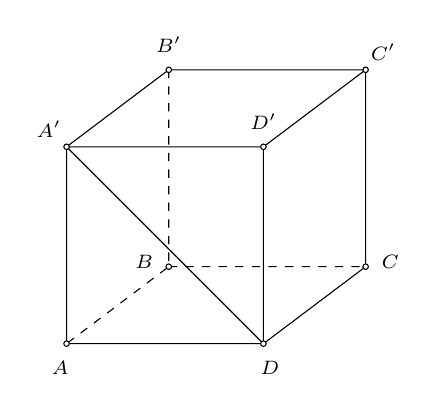
\begin{tikzpicture}[declare function={r=2.5;},font=\scriptsize]
				\path (0:0) coordinate (A)
				(0:r) coordinate (B)
				++(37:{0.65*r}) coordinate (C)
				++(180:r) coordinate (D)
				\foreach \x in {A,B,C,D}{(\x)++(90:r) coordinate (\x_1)};
				\draw[dashed] (D_1)--(D)--(A) (D)--(C);
				\draw (A)--(B)--(C) (A)--(A_1) (B)--(B_1) (C)--(C_1)(A_1)--(B_1)--(C_1)--(D_1)--cycle (A_1)--(B);
				\foreach \x/\goc/\t in {A/255/A, B/-75/D, C/10/C, D/170/B, A_1/135/A', B_1/90/D',
					C_1/45/C', D_1/90/B'}{
					\draw[fill=white] (\x) circle (1pt) node[shift={(\goc:9pt)}]{$\t$};
				}
			\end{tikzpicture}
		}
	}
\end{ex}
%%%=============================%%%

%%%=============EX_11=============%%%
\begin{ex}%[1H8H1-2]%[Dự án đề cương 3 Khối NH 24-25- Dot 2 - Nguyễn Trần Anh Tuấn]
	Cho hình hộp chữ nhật $ABCD.EFGH$. Khẳng định nào dưới đây đúng?
	\choice
	{$FB\perp AG$}
	{\True $AB\perp DH$}
	{$HD\perp BF$}
	{$CD\perp EG$}
	\loigiai{
		\immini {
			Ta có $\heva{&DC\perp DH\\&DC\parallel AB}\Rightarrow AB\perp DH$.
		}
		{
			\begin{tikzpicture}[declare function={a=3; b=0.45*a; h=0.65*a;}]
				\path (0:0) coordinate (A)
				(220:b) coordinate (B)
				($(B)+(a,0)$) coordinate (C)
				(a,0) coordinate (D)
				\foreach \x in {A,B,C,D}{(\x)++(90:h) coordinate (\x1)};
				\draw[dashed] (A1)--(A)--(B) (A)--(D);
				\draw (B1)--(A1)--(D1)--(C1) (D1)--(D)--(C) (B)--(C)--(C1)--(B1)--cycle;
				\foreach \x/\goc/\t in {A/180/B,B/-90/A,C/-90/D,D/0/C,A1/90/F,B1/90/E,C1/90/H,D1/90/G}
				\draw[fill=white] (\x) circle (1pt) node[shift={(\goc:7pt)},font=\scriptsize]{$\t$};
			\end{tikzpicture}
		}
	}
\end{ex}
%%%=============================%%%

%%%=============EX_12=============%%%
\begin{ex}%[1H8H1-2]%[Dự án đề cương 3 Khối NH 24-25- Dot 2 - Nguyễn Trần Anh Tuấn]
	Cho hình chóp $S.ABCD$ có đáy $ABCD$ là hình vuông. Gọi $M$, $N$ lần lượt là trung điểm của các cạnh $SA$ và $SC$. Khi đó đường thẳng $MN$ vuông góc với đường thẳng nào sau đây?
	\choice
	{$AC$}
	{$AD$}
	{\True $BD$}
	{$CD$}
	\loigiai{
		\immini{Xét $\triangle SAC$ ta có $\heva{&MA=MS\\&NC=NS}\Rightarrow MN$ là đường trung bình của $\triangle SAC$.\\
			Khi đó $MN\parallel AC$.\\
			Vì tứ giác $ABCD$ là hình vuông nên $AC\perp BD$.\\ Từ các kết quả trên, ta có $BD\perp MN$.}
		{\begin{tikzpicture}[declare function={gocx=80; goc=-150; a=4; b=a/2; h=4;}]
				\path (0,0) coordinate (A)--+(gocx:h) coordinate (S)
				(a,0) coordinate (D)
				(goc:b) coordinate (B)
				+(a,0) coordinate (C)
				($(A)!0.5!(S)$) coordinate (M)
				($(C)!0.5!(S)$) coordinate (N)
				;
				\draw[dashed] (S)--(A) (B)--(A)--(D) (M)--(N) (A)--(C) (B)--(D);
				\draw (S)--(B)--(C)--(S)--(D)--(C)--cycle;
				\foreach \x/\goc in {S/90,A/150,B/-90,C/-60,D/0,M/180,N/0}
				\draw[fill=white] (\x) node[shift={(\goc:7pt)},font=\scriptsize]{$\x$} circle (1pt);
			\end{tikzpicture}
		}
	}
\end{ex}
%%%=============================%%%

%%%=============EX_13=============%%%
\begin{ex}%[1H8H1-2]%[Dự án đề cương 3 Khối NH 24-25- Dot 2 - Nguyễn Trần Anh Tuấn]
	Cho hình hộp $ABCD.A'B'C'D'$ có tất cả các cạnh đều bằng nhau. Trong các mệnh đề sau, mệnh đề nào đúng?
	\choice
	{\True $A'C'\perp BD$}
	{$A'B'\perp BC$}
	{$CC'\perp AB$}
	{$BB'\perp BD$}
	\loigiai{
		\immini{
			Vì $ABCD$ là hình thoi nên $AC\perp BD$.\\ 
			Mà $A'C'\parallel AC$.\\ 
			Suy ra $A'C'\perp BD$.}
		{	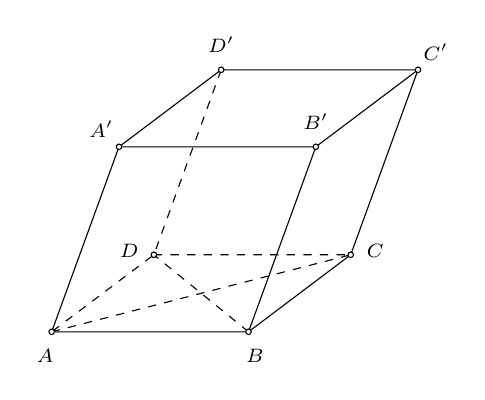
\begin{tikzpicture}[declare function={r=2.5;},font=\scriptsize]
				\path (0:0) coordinate (A)
				(0:r) coordinate (B)
				++(37:{0.65*r}) coordinate (C)
				++(180:r) coordinate (D)
				\foreach \x in {A,B,C,D}{(\x)++(70:r) coordinate (\x_1)};
				\draw[dashed] (D_1)--(D)--(A) (D)--(C) (A)--(C) (B)--(D);
				\draw (A)--(B)--(C) (A)--(A_1) (B)--(B_1) (C)--(C_1)(A_1)--(B_1)--(C_1)--(D_1)--cycle;
				\foreach \x/\goc/\t in {A/255/A, B/-75/B, C/10/C, D/170/D, A_1/135/A', B_1/90/B',
					C_1/45/C', D_1/90/D'}{
					\draw[fill=white] (\x) circle (1pt) node[shift={(\goc:9pt)}]{$\t$};
				}
			\end{tikzpicture}
		}
	}
\end{ex}
%%%=============================%%%

%%%=============EX_14=============%%%
\begin{ex}%[1H8H1-2]%[Dự án đề cương 3 Khối NH 24-25- Dot 2 - Nguyễn Trần Anh Tuấn]
	Cho hình hộp $ABCD.A’B’C’D’$ có tất cả các cạnh đều bằng nhau. Trong các mệnh đề sau, mệnh đề nào có thể {\bf sai}?
	\choice
	{$A’C’\perp BD$}
	{\True $BB’\perp BD$}
	{$A’B\perp DC’$}
	{$BC’\perp A'D$}
	\loigiai{
		\immini{
			\begin{itemize}
				\item
				$\heva{&A'C'\perp B'D'\\
					&B'D'\parallel BD\\
				}\Rightarrow A'C'\perp BD$.
				\item $\heva{&A'B\perp AB’\\
					&AB’\parallel DC’\\
				}\Rightarrow A'B\perp DC’$.
				\item $\heva{&BC’\perp B'C\\
					&B'C\parallel A’D\\
				}\Rightarrow BC’\perp A'D$.
			\end{itemize}
		}{
			\begin{tikzpicture}[line join=round,line cap=round, font=\footnotesize,scale=.7,>=stealth]
				\path
				(0,0) coordinate (B)
				(2,2) coordinate (A)
				(4,0) coordinate (C)
				(1,4) coordinate (B')
				($(C)+(B')$)coordinate (C')
				($(C)+(A)$)coordinate (D)
				($(B')+(A)$)coordinate (A')
				($(B')+(D)$)coordinate (D')
				;
				\draw
				(B)--(C)--(C')--(B')--(B)(C')--(D')--(A')--(B')(D)--(C')(C)--(D)--(D')(B')--(C)(A')--(C')(B')--(D') (B)--(C');
				\draw[dashed](B)--(A)--(D)--(B)(A')--(A)--(B')(A')--(D)--(B')(A)--(C) (A')--(B) (A')--(D);
				\foreach \x/\goc/\t in {A/180/A,B/180/B,C/0/C,D/0/D,A'/180/A',B'/180/B',C'/90/C',D'/0/D'}{
					\draw[fill=white] (\x) circle (1pt) node[shift={(\goc:9pt)}]{$\t$};
				}
			\end{tikzpicture}
		}
	}
\end{ex}
%%%=============================%%%

%%%=============EX_15=============%%%
\begin{ex}%[1H8H1-2]%[Dự án đề cương 3 Khối NH 24-25- Dot 2 - Nguyễn Trần Anh Tuấn]
	Cho hình chóp $S.ABCD$ có đáy là hình vuông
	$ABCD$ cạnh bằng $a$ và các cạnh bên đều bằng $a$. Gọi $M$ và $N$ lần lượt là trung điểm của $AD$ và $SD$. Đường thẳng $MN$ vuông góc với đường thẳng nào sau đây?
	\choice
	{$BD$}
	{\True $SC$}
	{$AC$}
	{$AD$}
	\loigiai{
		\immini{
			Ta có $\heva{&AC^{2}=2a^{2}\\
				&SA^{2}+SC^{2}=2a^{2}}
			\Rightarrow AC^{2}=SA^{2}+SC^{2}$.\\
			Suy ra $\triangle SAC$ vuông tại $S$ (định lý Pytago đảo).\\
			Ta có $MN$ là đường trung bình
			$\triangle SAD$.\\
			Suy ra $MN\parallel SA$, mà $SA\perp SC$.\\
			Do đó $MN\perp SC$.}
		{
			\begin{tikzpicture}[declare function={goc=-150; a=4; b=a/2; h=a;}]
				\path (0,0) coordinate (A)
				(a,0) coordinate (B)
				(goc:b) coordinate (D)
				+(a,0) coordinate (C)
				($(A)!.5!(C)$) coordinate (O)--+(0,h) coordinate (S)
				($(S)!0.5!(D)$) coordinate (N)
				($(A)!0.5!(D)$) coordinate (M);
				\draw pic[angle radius=3mm,draw] {right angle = S--O--D};
				\draw pic[angle radius=3mm,draw] {right angle = B--A--D};
				\draw[dashed] (S)--(A) (D)--(A)--(B) (S)--(O) (A)--(C) (D)--(B) (M)--(N);
				\draw (S)--(D)--(C)--(S)--(B)--(C)--cycle;
				\foreach \x/\goc in {S/90,A/150,B/0,C/-60,D/-180,O/-90,M/-10,N/150}
				\draw[fill=white] (\x) node[shift={(\goc:7pt)},font=\scriptsize]{$\x$} circle (1pt);
			\end{tikzpicture}
		}
	}
\end{ex}
%%%=============================%%%

%%%=============EX_16=============%%%
\begin{ex}%[1H8H1-3]%[Dự án đề cương 3 Khối NH 24-25- Dot 2 - Nguyễn Trần Anh Tuấn]
	Cho hình chóp $S.ABCD$ có tất cả các cạnh đều bằng $a$. Gọi $I$ và $J$ lần lượt là trung điểm của $SC$ và $BC$. Số đo của góc $\left(IJ,CD\right)$ bằng
	\choice
	{$30^{\circ}$}
	{$45^{\circ}$}
	{\True $60^{\circ}$}
	{$90^{\circ}$}
	\loigiai{
		\immini{
			Ta có $\heva{&IS=IC\\&JB=JC}$ suy ra $IJ$ là đường trung bình của $\triangle SBC$.\\
			Do đó $IJ\parallel SB$.\\
			Lại có $DC\parallel AB$.\\
			Suy ra $\left(IJ,CD\right)=\left(SB,AB\right)=\widehat{SBA}
			=60^{\circ}$ (do $\triangle SAB$ đều).
		}
		{
			\begin{tikzpicture}[declare function={goc=-150; a=4; b=a/2; h=a;}]
				\path (0,0) coordinate (A)
				(a,0) coordinate (B)
				(goc:b) coordinate (D)
				+(a,0) coordinate (C)
				($(A)!.5!(C)$) coordinate (O)--+(0,h) coordinate (S)
				($(S)!0.5!(C)$) coordinate (I)
				($(C)!0.5!(B)$) coordinate (J);
				\draw pic[angle radius=3mm,draw] {right angle = S--O--D};
				\draw pic[angle radius=3mm,draw] {right angle = B--A--D};
				\draw[dashed] (S)--(A) (D)--(A)--(B) (S)--(O) (A)--(C) (D)--(B);
				\draw (S)--(D)--(C)--(S)--(B)--(C)--cycle (I)--(J);
				\foreach \x/\goc in {S/90,A/150,B/0,C/-60,D/-180,O/-90,I/180,J/0}
				\draw[fill=white] (\x) node[shift={(\goc:7pt)},font=\scriptsize]{$\x$} circle (1pt);
			\end{tikzpicture}
		}
	}
\end{ex}
%%%=============================%%%

%%%=============EX_17=============%%%
\begin{ex}%[1H8H1-3]%[Dự án đề cương 3 Khối NH 24-25- Dot 2 - Nguyễn Trần Anh Tuấn]
	Cho hình chóp $S.ABC$ có $SA$, $SB$, $SC$ đôi một vuông góc với nhau và $SA=SB=SC=a$. Gọi $M$ là trung điểm $AB$. Tính góc giữa hai đường thẳng $SM$ và $BC$.
	\choice
	{$30^{\circ}$}
	{\True $60^{\circ}$}
	{$90^{\circ}$}
	{$120^{\circ}$}
	\loigiai{
		\immini{
			Ta có $AB=BC=CA=a\sqrt{2}$.\\
			Gọi $ N$ là trung điểm $ AC$.\\
			Khi đó
			$\heva{&MN=\dfrac{BC}{2}\\&SM=\dfrac{AB}{2}\\&SN=\dfrac{AC}{2}}\Rightarrow MN=SM=SN$.\\
			Suy ra $\triangle SMN$ đều
			$\Rightarrow\widehat{NMS}=60^{\circ}$.\\
			Lại có
			$MN\parallel BC\Rightarrow(SM,BC)=(SM,MN)=\widehat{NMS}=60^{\circ}$.
		}{
			\begin{tikzpicture}[declare function={goc=-45; a=5; b=0.4*a; h=3;}]
				\path
				(0,0) coordinate (S)--+(0,h) coordinate (C)
				(a,0) coordinate (B)
				(goc:b) coordinate (A)
				($(A)!0.5!(B)$) coordinate (M)
				($(A)!0.5!(C)$) coordinate (N);
				\draw
				pic[angle radius=3mm,draw] {right angle = B--S--C}
				pic[angle radius=3mm,draw] {right angle = A--S--C}
				pic[angle radius=3mm,draw] {right angle = A--S--B}
				;
				\draw[dashed] (S)--(B) (S)--(M);
				\draw (S)--(A)--(B)--(C)--cycle (A)--(C) (M)--(N)--(S);
				\foreach \x/\goc in {S/180,A/-60,C/90,B/0,M/-30,N/180}
				\draw[fill=white] (\x) node[shift={(\goc:7pt)},font=\scriptsize]{$\x$} circle (1pt);
			\end{tikzpicture}
		}
	}
\end{ex}
%%%=============================%%%

%%%=============EX_18=============%%%
\begin{ex}%[1H8H1-3]%[Dự án đề cương 3 Khối NH 24-25- Dot 2 - Nguyễn Trần Anh Tuấn]
	Cho tứ diện đều $ABCD$ cạnh $a$. Tính cosin góc giữa hai đường thẳng $AB$ và $CI$ với $I$ là trung điểm của $AD$.
	\choice
	{\True $\dfrac{\sqrt{3}}{6}$}
	{$\dfrac{1}{2}$}
	{$\dfrac{\sqrt{3}}{4}$}
	{$\dfrac{\sqrt{3}}{2}$}
	\loigiai{
		\immini{
			Gọi $M$ là trung điểm $BD$.\\ 
			Khi đó $MI\parallel AB$.\\
			Suy ra $(AB,CI)=(MI,CI)=\widehat{CIM}$.\\
			Ta có $CI=CM=\dfrac{a\sqrt{3}}{2}$, $MI=\dfrac{AB}{2}=\dfrac{a}{2}$.\\
			$\cos CIM=\dfrac{IC^2+IM^2-CM^2}{2\cdot IC\cdot IM}=\dfrac{\dfrac{a^2}{4}}{2\cdot\dfrac{a\sqrt{3}}{2}\cdot\dfrac{a}{2}}=\dfrac{\sqrt{3}}{6}$.
		}{
			\begin{tikzpicture}[declare function={r=2.5;}]
				\path (90:{r*1.25}) coordinate (A)
				(160:{r} and {r*0.35}) coordinate (B)
				(20:{r} and {r*0.35}) coordinate (D)
				(260:{r} and {r*0.5}) coordinate (C)
				($(A)!0.5!(D)$) coordinate (I)
				($(D)!0.5!(B)$) coordinate (M);
				\draw[dashed] (B)--(D) (C)--(M)--(I);
				\draw (A)--(B)--(C)--(D) (A)--(C)--(I) (A)--(D);
				\foreach \x/\goc in {A/90,B/120,C/-90,D/-90,I/90,M/100}
				\draw[fill=white] (\x) node[shift={(\goc:7pt)},font=\scriptsize]{$\x$} circle (1pt);
			\end{tikzpicture}
		}
	}
\end{ex}
%%%=============================%%%

%%%=============EX_19=============%%%
\begin{ex}%[1H8H1-3]%[Dự án đề cương 3 Khối NH 24-25- Dot 2 - Nguyễn Trần Anh Tuấn]
	Cho tứ diện $ABCD$. Gọi $M$, $N$ lần lượt là trung điểm của $BC$ và $AD$. Biết $AB=CD=a$, $MN=\dfrac{a\sqrt{3}}{2}$. Tính góc giữa hai đường thẳng $AB$ và $CD$.
	\choice
	{$45^{\circ}$}
	{$30^{\circ}$}
	{\True $60^{\circ}$}
	{$90^{\circ}$}
	\loigiai{
		\immini{Gọi $P$ là trung điểm $AC$.\\
			Ta có $\heva{&MB=MC\\&PA=PC}\Rightarrow MP$ là đường trung bình của $\triangle ABC$.\\
			Suy ra $MP\parallel AB$.\\
			Tương tự $NP\parallel CD$.\\
			Khi đó $(AB,CD)=(MP,NP)=\widehat{MPN}$.\\
			\\
			Xét $\triangle MNP$ ta có $\cos MPN=\dfrac{MP^2+NP^2-MN^2}{2MP\cdot NP}=-\dfrac{1}{2}$.\\Suy ra $\widehat{MPN}=120^{\circ}$.\\ Do đó góc giữa hai đường thẳng $AB$ và $CD$ bằng $60^{\circ}$.}
		{
			\begin{tikzpicture}[declare function={goc=-55; a=4; b=0.45*a; h=5;}]
				\path
				(0,0) coordinate (B)
				(a,0) coordinate (D)
				(goc:b) coordinate (C)--+(0,h) coordinate (A)
				($(C)!0.5!(B)$) coordinate (M)
				($(A)!0.5!(C)$) coordinate (P)
				($(A)!0.5!(D)$) coordinate (N);
				\draw[dashed] (B)--(D) (M)--(N);
				\draw (A)--(B)--(C)--(D)--cycle (A)--(C) (M)--(P)--(N);
				\foreach \x/\goc in {A/90,C/-60,B/180,D/0,M/180,P/180,N/0}
				\draw[fill=white] (\x) node[shift={(\goc:7pt)},font=\scriptsize]{$\x$} circle (1pt);
			\end{tikzpicture}
		}
	}
\end{ex}
%%%=============================%%%

%%%=============EX_20=============%%%
\begin{ex}%[1H8H1-3]%[Dự án đề cương 3 Khối NH 24-25- Dot 2 - Nguyễn Trần Anh Tuấn]
	Cho tứ diện $ABCD$ có $AB=CD=a$. Gọi $M$ và $N$ lần lượt là trung điểm của $AD$ và $BC$. Xác định độ dài đoạn thẳng $MN$ để góc giữa hai đường thẳng $AB$ và $MN$ bằng $30^{\circ}$.
	\choice
	{$MN=\dfrac{a}{2}$}
	{\True $MN=\dfrac{a\sqrt{3}}{2}$}
	{$MN=\dfrac{a\sqrt{3}}{3}$}
	{$MN=\dfrac{a}{4}$}
	\loigiai{
		\immini{
			Gọi $P$ là trung điểm của $AC$.\\
			Suy ra $PM=\dfrac{1}{2}CD=\dfrac{1}{2}AB=PN$.\\
			Do đó $\triangle PMN$ cân tại $P$.\\
			Lại có $(AB,MN)=30^{\circ}$ nên $(MN,PN)=30^{\circ}$.\\
			Vậy $\triangle PMN$ là tam giác cân có góc ở đỉnh bằng $120^{\circ}$.\\
			Ta có $PN\cdot\sqrt{3}=MN$ nên $MN=\dfrac{a\sqrt{3}}{2}$.}
		{
			
			\begin{tikzpicture}[declare function={goc=-45; a=5; b=0.4*a; h=5;}]
				\path
				(0,0) coordinate (D)
				(a,0) coordinate (C)
				(goc:b) coordinate (B)--+(0,h) coordinate (A)
				($(A)!0.5!(D)$) coordinate (M)
				($(B)!0.5!(C)$) coordinate (N)
				($(A)!0.5!(C)$) coordinate (P)
				;
				\draw[dashed] (D)--(C) (P)--(M)--(N);
				\draw (A)--(B)--(D)--cycle (A)--(B)--(C)--cycle (N)--(P);
				\foreach \x/\goc in {D/180,A/90,C/0,B/-90,M/180,N/-30,P/0}
				\draw[fill=white] (\x) node[shift={(\goc:7pt)},font=\scriptsize]{$\x$} circle (1pt);
			\end{tikzpicture}
		}
	}
\end{ex}
%%%=============================%%%


\ind{PHẦN II.} \inden{Câu trắc nghiệm đúng sai. Trong mỗi ý a), b), c), d) ở mỗi câu, học sinh chọn đúng hoặc sai.}\\
\setcounter{ex}{0}
\Opensolutionfile{ans}[ans/1H8-Bai1-DS]
%%%=============EX_1=============%%%
\begin{ex}%[1H8H2-1]%[Dự án đề cương 3 Khối NH 24-25- Dot 2 - Nguyễn Trần Anh Tuấn]
	\immini{Cho hình chóp $S.ABCD$ có đáy là hình thoi cạnh $a$.\\ Cho biết $SA=a\sqrt{3}$, $SA\perp AB$, $SA\perp AD$.
		\choiceTF
		{\True $(AB,SA)=90^{\circ}$}
		{\True $SA\perp CD$}
		{$(SD,BC)=(SD,CD)$}
		{\True $\widehat{SDA}=60^{\circ}$}}
	{\begin{tikzpicture}
			\tikzset{declare function={a=3; b=2; h=2.5;}}
			\path (0,0) coordinate (A)
			(a,0) coordinate (B)
			(-135:b) coordinate (D)
			($(B)+(D)$) coordinate (C)
			(0,h) coordinate (S)
			($(S)!0.5!(D)$) coordinate (M)
			($(S)!0.5!(B)$) coordinate (N);
			\path pic[draw,angle radius=5pt]{right angle=D--A--S};
			\path pic[draw,angle radius=5pt]{right angle=B--A--S};
			\draw[dashed] (B)--(A)--(D) (A)--(S) (A)--(C) (B)--(D) (M)--(N);
			\draw (S)--(D)--(C)--(B)--cycle (S)--(C);
			\foreach \t/\g in {A/180,B/0,C/0,D/180,S/90,M/180,N/30}{
				\draw[fill=white] (\t) circle (1pt) node[shift={(\g:9pt)},font=\scriptsize]{$\t$};
			}
	\end{tikzpicture}}
	\loigiai{
		\begin{itemchoice}
			\itemch Vì $SA\perp AB$ nên $(AB,SA)=90^{\circ}$.
			\itemch Vì $\heva{&SA\perp AB\\&AB\parallel CD}$ nên suy ra $SA\perp CD$.
			\itemch Vì $BC\parallel AD$ nên $(SD,BC)=(SD,AD)$.
			\itemch Xét $\triangle SAD$ vuông tại $A$ ta có
			$\tan SDA=\dfrac{SA}{AD}=\dfrac{a\sqrt{3}}{a}=\sqrt{3}$.
			Suy ra $\widehat{SDA}=60^{\circ}$.
		\end{itemchoice}
	}
\end{ex}
%%%=============================%%%

%%%=============EX_2=============%%%
\begin{ex}[Trích đề thi GHKII - THPT Edison, Hải Phòng - Năm học: 2024-2025]%[1H8H1-3]%[Dự án đề cương 3 Khối NH 24-25- Dot 2 - Nguyễn Trần Anh Tuấn]
	\immini{Cho hình lập phương $ABCD.A'B'C'D'$.
		\choiceTF
		{\True $AC\perp B'D'$}
		{Góc giữa hai đường thẳng $B'D'$ và $AA'$ bằng $60^{\circ}$}
		{\True Góc giữa hai đường thẳng $AB$ và $D'C$ bằng $45^{\circ}$}
		{$D'C\perp A'C'$}}
	{\begin{tikzpicture}[font=\footnotesize,line join=round, line cap=round, >=stealth,scale=0.8]
			\path
			(0,0) coordinate (B)
			($(B)+(0:3)$) coordinate (C)
			($(B)+(20:2)$) coordinate (A)
			($(A)+(C)-(B)$) coordinate (D)
			($(A)+(90:3)$) coordinate (A')
			($(A')+(B)-(A)$) coordinate (B')
			($(B')+(C)-(B)$) coordinate (C')
			($(A')+(D)-(A)$) coordinate (D');
			\draw (B)--(B')--(C')--(C)--(B) (B')--(A')--(D')--(D)--(C) (C')--(D') (C)--(D') (C')--(A') (B')--(D');
			\draw[dashed] (B)--(A)--(D)--(C) (A)--(A')--(B)--(D) (C)--(A);
			\foreach \x/\goc in {B/-150,C/-90,A'/90,D/0,A/150,B'/150,C'/-30,D'/0}
			\draw[fill=white] (\x) node[shift={(\goc:7pt)},font=\scriptsize]{$\x$} circle (1pt);
	\end{tikzpicture}}
	\loigiai{
		\immini{
			\begin{itemchoice}
				\itemch Ta có $\heva{&AC\perp BD\\&BD\parallel B'D'}\Rightarrow AC\perp B'D'$.
				\itemch $AA'\perp\left(A'B'C'D'\right)\Rightarrow AA'\perp B'D'$. Do đó $(AA',B'D')=90^{\circ}$.
				\itemch Do $AB\parallel CD$ nên $(AB,CD')=(CD,CD')=\widehat{DCD'}=45^{\circ}$.
				\itemch Do $A'C'\parallel AC$ nên $(A'C',D'C)=(AC,D'C)=60^{\circ}$ (do $\triangle ACD'$ đều).
		\end{itemchoice}}
		{\begin{tikzpicture}[font=\footnotesize,line join=round, line cap=round, >=stealth,scale=0.8]
				\path
				(0,0) coordinate (B)
				($(B)+(0:3)$) coordinate (C)
				($(B)+(20:2)$) coordinate (A)
				($(A)+(C)-(B)$) coordinate (D)
				($(A)+(90:3)$) coordinate (A')
				($(A')+(B)-(A)$) coordinate (B')
				($(B')+(C)-(B)$) coordinate (C')
				($(A')+(D)-(A)$) coordinate (D');
				\draw (B)--(B')--(C')--(C)--(B) (B')--(A')--(D')--(D)--(C) (C')--(D') (C)--(D') (C')--(A') (B')--(D') ;
				\draw[dashed] (B)--(A)--(D)--(C) (A)--(A')--(B)--(D) (C)--(A) (A)--(D');
				\foreach \x/\goc in {B/-150,C/-90,A'/90,D/0,A/150,B'/150,C'/-30,D'/0}
				\draw[fill=white] (\x) node[shift={(\goc:7pt)},font=\scriptsize]{$\x$} circle (1pt);
		\end{tikzpicture}}
	}
\end{ex}
%%%=============================%%%

%%%=============EX_3=============%%%
\begin{ex}%[1H8H1-3]%[Dự án đề cương 3 Khối NH 24-25- Dot 2 - Nguyễn Trần Anh Tuấn]
	\immini{Cho hình lập phương $ABCD.A'B'C'D'$ có cạnh bằng $a$. Gọi $O$ là giao điểm của $AC$, $BD$.
		\choiceTF
		{\True Hai đường thẳng $BB'$ và $C'D'$ vuông góc với nhau}
		{Góc giữa hai đường thẳng $A'C'$ và $AB$ bằng $60^{\circ}$}
		{\True Góc giữa hai đường thẳng $A'C'$ và $CD'$ bằng $60^{\circ}$}
		{Hai đường thẳng $A'O$ và $CD'$ vuông góc với nhau}}
	{\begin{tikzpicture}[>=stealth,line join=round,line cap=round,font=\footnotesize,scale=0.85]
			\def\r{-150}
			\def\c{3}
			\def\d{1.3}
			\path
			(0:0) coordinate (A)++(0:\c)
			coordinate (D)++(90:\c)coordinate(D')
			(A)++(\r:\d) coordinate (B)++(0:\c) coordinate (C)++(90:\c)coordinate(C')
			(A)++(90:\c) coordinate (A')++(\r:\d) coordinate (B')
			(intersection of A--C and B--D) coordinate (O)% Giao điểm của hai đường thẳng
			;
			\draw (C')--(A')--(B')--(B)--(C)--(D)--(D')--(A') (C)--(C')--(B) (B')--(C')--(D') (C)--(D');
			\draw[dashed] (A')--(A)--(D) (C)--(A)--(B)--(A') (A')--(O);
			\foreach \x/\goc in {A/45,B/-135,D/0,A'/135,B'/135,D'/45,C/-90,C'/90,O/220}
			\draw[fill=white] (\x) node[shift={(\goc:7pt)},font=\scriptsize]{$\x$} circle (1pt);
			\draw pic[draw=black,angle radius=0.2cm] {angle = B'--A'--C'};
			\draw pic[draw,double,angle eccentricity=1.2,angle radius=0.3cm]{angle=B--A'--C'};
	\end{tikzpicture}}
	\loigiai{
		\immini{
			\begin{itemchoice}
				\itemch Ta có $\left(BB', C'D'\right)=\left(BB',B'A'\right)=90^{\circ}$ nên hai đường thẳng $BB'$ và $C'D'$ vuông góc với nhau.
				\itemch Ta có $\left(A'C', AB\right)=\left(A'C', A'B'\right)=\widehat{B'A'C'}=45^{\circ}$ do $A'B'C'D'$ là hình vuông.\\
				Vậy góc giữa hai đường thẳng $A'C'$ và $AB$ bằng $45^{\circ}$.
				\itemch Ta có $\left(A'C',CD'\right)=\left(A'C', A'B\right)=60^{\circ}$ do $\triangle BA'C'$ là tam giác đều.\\
				Vậy góc giữa hai đường thẳng $A'C'$ và $CD'$ bằng $60^{\circ}$.
				\itemch Do $\triangle BA'D$ là tam giác đều, $O$ là trung điểm $BD$ nên $A'O\perp BD$ $\Rightarrow\widehat{BA'O}<90^{\circ}$.\\
				Ta có $\left(A'O, CD'\right)=\left(A'O, A'B\right)=\widehat{BA'O}$.\\
				Vậy hai đường thẳng $A'O$ và $CD'$ không thể vuông góc với nhau.
		\end{itemchoice}}
		{\begin{tikzpicture}[>=stealth,line join=round,line cap=round,font=\footnotesize,scale=0.85]
				\def\r{-150}
				\def\c{3}
				\def\d{1.3}
				\path
				(0:0) coordinate (A)++(0:\c)
				coordinate (D)++(90:\c)coordinate(D')
				(A)++(\r:\d) coordinate (B)++(0:\c) coordinate (C)++(90:\c)coordinate(C')
				(A)++(90:\c) coordinate (A')++(\r:\d) coordinate (B')
				(intersection of A--C and B--D) coordinate (O)% Giao điểm của hai đường thẳng
				;
				\draw (C')--(A')--(B')--(B)--(C)--(D)--(D')--(A') (C)--(C')--(B) (B')--(C')--(D') (C)--(D');
				\draw[dashed] (A')--(A)--(D) (C)--(A)--(B)--(A') (A')--(O) (B)--(D)--(A');
				\foreach \x/\goc in {A/45,B/-135,D/0,A'/135,B'/135,D'/45,C/-90,C'/90,O/220}
				\draw[fill=white] (\x) node[shift={(\goc:7pt)},font=\scriptsize]{$\x$} circle (1pt);
				\draw pic[draw=black,angle radius=0.2cm] {angle = B'--A'--C'};
				\draw pic[draw,double,angle eccentricity=1.2,angle radius=0.3cm]{angle=B--A'--C'};
			\end{tikzpicture}
		}
	}
\end{ex}
%%%=============================%%%

%%%=============EX_4=============%%%
\begin{ex}%[1H8H1-3]%[Dự án đề cương 3 Khối NH 24-25- Dot 2 - Nguyễn Trần Anh Tuấn]
	\immini{Cho hình chóp $S.ABCD$ có đáy là hình thoi. Gọi $M$, $N$ theo thứ tự là trung điểm của đoạn $SB$, $SD$.
		\choiceTF
		{\True $MN\parallel BD$}
		{\True $MN$ và $AC$ là hai đường thẳng chéo nhau}
		{\True $AC\perp BD$}
		{\True $(MN,AC)=90^{\circ}$}}
	{\begin{tikzpicture}
			\tikzset{declare function={a=3; b=2; h=2.5;}}
			\path (0,0) coordinate (A)
			(a,0) coordinate (D)
			(-135:b) coordinate (B)
			($(B)+(D)$) coordinate (C)
			(0,h) coordinate (S)
			($(S)!0.5!(B)$) coordinate (M)
			($(S)!0.5!(D)$) coordinate (N);
			\path pic[draw,angle radius=5pt]{right angle=B--A--S};
			\path pic[draw,angle radius=5pt]{right angle=D--A--S};
			\draw[dashed] (B)--(A)--(D) (A)--(S) (A)--(C) (B)--(D) (M)--(N);
			\draw (S)--(B)--(C)--(D)--cycle (S)--(C);
			\foreach \t/\g in {A/180,B/-90,C/-90,D/90,S/90,M/180,N/30}{
				\draw[fill=white] (\t) circle (1pt) node[shift={(\g:9pt)},font=\scriptsize]{$\t$};
			}
	\end{tikzpicture}}
	\loigiai{
		\begin{itemchoice}
			\itemch $\triangle SBD$ có $MN$ là đường trung bình nên suy ra $MN\parallel BD$.
			\itemch $MN$ và $AC$ không cùng nằm trên một mặt phẳng nên là hai đường thẳng chéo nhau.
			\itemch $ABCD$ là hình thoi nên $AC\perp BD$.
			\itemch Vì $MN\parallel BD$ nên $(MN,AC)=(BD,AC)=90^{\circ}$.
		\end{itemchoice}
	}
\end{ex}
%%%=============================%%%

%%%=============EX_5=============%%%
\begin{ex}%[1H8V1-3]%[Dự án đề cương 3 Khối NH 24-25- Dot 2 - Nguyễn Trần Anh Tuấn]
	\immini{Cho hình chóp $S.ABCD$ có đáy $ABCD$ là hình thang vuông tại $A$ và $D$. Gọi $E$ là trung điểm của $AB$. Biết $AB=2a$, $AD=DC=a$, đồng thời $SA\perp AB$, $SA\perp AD$ và $SA=\dfrac{2a\sqrt{3}}{3}$.
		\choiceTF
		{\True $(SB,DC)=\widehat{SBA}$}
		{$\tan SBA=\dfrac{\sqrt{3}}{2}$}
		{\True $DE\parallel BC$}
		{$(SD,BC)\approx 52{,}42^{\circ}$}}
	{\begin{tikzpicture}[line cap=round,line join=round,font=\footnotesize,>=stealth,scale=1]
			\fill (0,0) coordinate (A)
			(0:4) coordinate (B)
			(90:2) coordinate (S)
			(-65:1.75) coordinate (C)
			($(A)+(C)-0.5*(B)$) coordinate (D)
			($0.5*(B)$) coordinate (E);
			\draw (S)--(B)--(C) (D)--(S)--(C)--(D);
			\draw[dashed] (C)--(E)--(D)--(A)--(S) (A)--(B) (S)--(E);
			\foreach \t/\g in {A/180,B/0,C/-10,D/180,E/90,S/90}{
				\draw[fill=white] (\t) circle (1pt) node[shift={(\g:9pt)},font=\scriptsize]{$\t$};
			}
	\end{tikzpicture}}
	\loigiai{
		\begin{itemchoice}
			\itemch Vì $CD\parallel AB$ $\Rightarrow(SB,DC)=(SB,AB)=\widehat{SBA}$.
			\itemch Xét $\triangle SAB$ vuông tại $A$ ta có
			$\tan SBA=\dfrac{SA}{AB}=\dfrac{\dfrac{2a\sqrt{3}}{3}}{2a}=\dfrac{\sqrt{3}}{3}$.
			\itemch Vì $BE\parallel CD$, $BE=CD=a$ nên $BCDE$ là hình bình hành. Suy ra $DE\parallel BC$.
			\itemch Do $DE\parallel BC$ nên $(SD,BC)=(SD,DE)$.\\
			Ta có $SE^2=SA^2+AE^2=\dfrac{4a^2}{3}+a^2=\dfrac{7a^2}{3}$;\\ $SD^2=SA^2+AD^2=\dfrac{7a^2}{3}$; $DE^2=AD^2+AE^2=2a^2$.\\
			Suy ra $SE=SD=\dfrac{a\sqrt{21}}{3}$, $DE=a\sqrt{2}$.\\
			Áp dụng định lí cosin cho $\triangle SDE$ ta được
			\[\cos SDE=\dfrac{SD^2+DE^2-SE^2}{2SD \cdot DE}=\dfrac{2a^2}{2 \cdot \dfrac{a\sqrt{21}}{3} \cdot a\sqrt{2}}=\dfrac{\sqrt{42}}{14}>0.\]
			Vậy $(SD,BC)=(SD,DE)=\widehat{SDE}\approx 62{,}42^{\circ}$.
		\end{itemchoice}
	}
\end{ex}
%%%=============================%%%

\ind{PHẦN III.} \inden{Trả lời ngắn.}\\
\setcounter{ex}{0}
\Opensolutionfile{ans}[ans/1H8-Bai1-KQ]

%%%=============EX_1=============%%%
\begin{ex}[Trích đề thi HKII - THPT Lê Lợi, Kon Tum - năm học 2024-2025]%[1H8V1-3]
	Cho hình tứ diện $S.ABC$ có tất cả các cạnh bằng nhau và bằng $a$. Điểm $K$ thuộc cạnh $SB$ sao cho $SK=\dfrac{2}{3}SB$. Tính côsin của góc giữa hai đường thẳng $AB$ và $CK$ (\textit{làm tròn đến chữ số thập phân thứ hai}).
	
	\shortans[oly]{0{,}37}
	\loigiai{
		\begin{center}
			\begin{tikzpicture}[scale=1, font=\footnotesize, line join=round, line cap=round, >=stealth]
				\def\ac{4} % cạnh AC
				\def\ab{2} % cạnh AB
				\def\h{4} % chiều cao
				\def\gocA{50} % góc A của đáy
				\coordinate[label=left:$A$] (A) at (0,0);
				\coordinate[label=right:$C$] (C) at (\ac,0);
				\coordinate[label=below left:$B$] (B) at (-\gocA:\ab);
				\coordinate[label=above:$S$] (S) at ($(A)+(70:\h)$);
				\coordinate[label=above right:$K$] (K) at ($(S)!2/3!(B)$);
				\coordinate[label=above left:$I$] (I) at ($(S)!2/3!(A)$);
				% \coordinate[label=above right:$H$] (H) at ($(S)!0.5!(B)$);
				\draw (A)--(B)--(C)--(S)--(A) (S)--(B) (I)--(K)--(C);
				\draw[dashed] (A)--(C) (I)--(C);
				\foreach \diem in {A,B,C,S,I,K}	\fill (\diem)circle(1pt);
			\end{tikzpicture}	
		\end{center}
		Trong $(SAB)$ gọi $I\in SA$ sao cho $KI\parallel AB \Rightarrow \dfrac{SI}{SA}=\dfrac{2}{3}$. Do đó $(AB,KC)=(IK,KC)$.\\
		Xét tam giác $BKC$, áp dụng định lí côsin có:
		\begin{eqnarray*}
			KC^2&=&KB^2+BC^2-2\cdot KB\cdot BC\cdot\cos\widehat{KBC}\\
			&=&\left(\dfrac{a}{3}\right)^2+a^2-2\cdot \dfrac{a}{3}\cdot a\cdot\cos 60^{\circ}\\
			&=&\dfrac{7a^2}{9} \Rightarrow KC=\dfrac{a\sqrt{7}}{3}.	
		\end{eqnarray*}
		Tương tự tính được $IC=\dfrac{a\sqrt{7}}{3}$; $IK=\dfrac{2a}{3}$.\\
		Áp dụng định lí côsin cho tam giác $IKC$ có 
		$$\cos\widehat{IKC}=\dfrac{IK^2+KC^2-IC^2}{2\cdot IK\cdot KC}=\dfrac{\left(\dfrac{a\sqrt{7}}{3}\right)^2+\left(\dfrac{2a}{3}\right)^2-\left(\dfrac{a\sqrt{7}}{3}\right)^2}{2\cdot\dfrac{a\sqrt{7}}{3} \cdot\dfrac{2a}{3}}=\dfrac{\sqrt{7}}{7}.$$
		Vậy $\cos(AB,KC)=\dfrac{\sqrt{7}}{7}$.
	}
\end{ex}
%%%=============================%%%

%%%=============EX_2=============%%%
\begin{ex}%[1H8V1-3]%[Dự án đề cương 3 Khối NH 24-25- Dot 2 - Nguyễn Trần Anh Tuấn]
	Cho tứ diện đều $ABCD$ cạnh $2$. Gọi $M$ là trung điểm của $BC$. Tính góc giữa hai đường thẳng $DM$ và $AB$ (\textit{kết quả theo đơn vị độ và làm tròn đến độ}).
	\par
	\shortans[oly]{73}
	\loigiai{
		\immini{
			Gọi $N$ là trung điểm $AC$.\\ Khi đó $MN$ là đường trung bình của $\triangle ABC$ nên $MN\parallel AB$.\\
			Do đó $(DM,AB)=(DM,MN)=\widehat{NMD}$.\\
			Xét $\triangle MND$ ta có $\heva{&DM=DN=\sqrt{3}\text{(chiều cao của tam giác đều cạnh $a$)}\\&MN=\dfrac{AB}{2}=1\text{($MN$ là đường trung bình của $\triangle ABC$)}}$\\
			$$\Rightarrow\cos NMD=\dfrac{MN^2+MD^2-ND^2}{2MN\cdot MD}=\dfrac{\sqrt{3}}{6}\Rightarrow\widehat{NMD}\approx 73^{\circ}.$$
			Vậy $(DM,AB)=\widehat{NMD}\approx 73^{\circ}$.
		}{
			\begin{tikzpicture}[line join=round, line cap=round,every node/.style={scale=0.8}]
				\path
				(0,0) coordinate (B)
				(4,0) coordinate (D)
				(3,-1) coordinate (C)
				($(C)!.5!(B)$) coordinate (M)
				--+(0,3) coordinate (A)
				($(A)!.5!(C)$) coordinate (N);
				\draw (A)--(B)--(C)--(D)--cycle(M)--(A)--(C) (M)--(N)--(D);
				\draw[dashed] (B)--(D) (M)--(D);
				\foreach \t/\g in {A/90,B/180,C/-90,D/0,M/-90,N/75}{
					\draw[fill=white] (\t) circle (1pt) node[shift={(\g:9pt)},font=\scriptsize]{$\t$};
				}
			\end{tikzpicture}
		}
	}
\end{ex}
%%%=============================%%%

%%%=============EX_3=============%%%
\begin{ex}[Trích đề thi HKII - THPT Lê Quý Đôn, Ninh Thuận - năm học 2024-2025]%[1H8V1-3]%[Dự án đề cương 3 Khối NH 24-25- Dot 2 - Nguyễn Trần Anh Tuấn]
	\immini{
		Cho hình lăng trụ $ABC.A'B'C'$ có đáy $ABC$ là tam giác đều cạnh a. Điểm $H$ là trung điểm cạnh $BC$, $A'H\perp(ABC)$ và $A'H=\dfrac{3a}{2}$ (tham khảo hình vẽ). Gọi $\alpha$ là góc giữa hai đường thẳng $CC'$ và $AB$. Khi đó, $\cos\alpha$ bằng $\sqrt{\dfrac{a}{b}}$, $\left(\dfrac{a}{b}\text{là phân số tối giản}\right)$. Hiệu $a-b$ bằng bao nhiêu?
	}
	{
		\begin{tikzpicture}[scale=.7, font=\footnotesize, line join=round, line cap=round, >=stealth]
			\def\ac{4} \def\ab{2} \def\h{4.0} \def\gocA{50}
			\coordinate (A) at (0,0);
			\coordinate (C) at (\ac,0);
			\coordinate (B) at (-\gocA:\ab);
			\coordinate (A') at ($(A)+(50:\h)$);
			\coordinate (B') at ($(B)-(A)+(A')$);
			\coordinate (C') at ($(C)-(A)+(A')$);
			\coordinate (H) at ($(B)!0.5!(C)$);
			\draw (A')--(A)--(B)--(C)--(C')--(A')--(B')--(C') (B)--(B');
			\draw[dashed] (A)--(C);
			\draw [dashed] (A')--(H);
			\foreach \t/\g in {A/180,B/-90,C/0,A'/90,B'/-90,C'/90,H/-90}{
				\draw[fill=white] (\t) circle (1pt) node[shift={(\g:9pt)},font=\scriptsize]{$\t$};
			}
		\end{tikzpicture}
	}
	\par
	\shortans[oly]{-13}
	\loigiai{
		\immini{Do $CC'\parallel AA'$ nên $(CC',AB)=(AA',AB)$.\\
			Ta có\\
			$AB=a$, $AA'=\sqrt{A'H^2+AH^2}=\sqrt{\dfrac{9a^2}{4}+\dfrac{3a^2}{4}}=a\sqrt{3}.$\\ $A'B=\sqrt{A'H^2+BH^2}=\sqrt{\dfrac{9a^2}{4}+\dfrac{a^2}{4}}=\dfrac{a\sqrt{10}}{2}$.\\
			Áp dụng định lí cosin trong $\triangle AA'B$ có\\
			$\cos BAA'=\dfrac{AB^2+AA'^2-A'B^2}{2\cdot AB\cdot AA'}=\dfrac{a^2+3a^2-\dfrac{10a^2}{4}}{2\cdot a\cdot a\sqrt{3}}=\sqrt{\dfrac{3}{16}}>0.\\
			\Rightarrow\cos(CC',AB)=\cos BAA'=\sqrt{\dfrac{3}{16}}\Rightarrow a-b=3-16=-13$.}
		{\begin{tikzpicture}[scale=.7, font=\footnotesize, line join=round, line cap=round, >=stealth]
				\def\ac{4} \def\ab{2} \def\h{4.0} \def\gocA{50}
				\coordinate (A) at (0,0);
				\coordinate (C) at (\ac,0);
				\coordinate (B) at (-\gocA:\ab);
				\coordinate (A') at ($(A)+(50:\h)$);
				\coordinate (B') at ($(B)-(A)+(A')$);
				\coordinate (C') at ($(C)-(A)+(A')$);
				\coordinate (H) at ($(B)!0.5!(C)$);
				\draw (H)--++(90:0.25)--++(-195 :0.15)--++(-90:0.25);
				\draw (B)--(A')--(A)--(B)--(C)--(C')--(A')--(B')--(C') (B)--(B');
				\draw[dashed] (H)--(A)--(C) (A')--(H);
				\foreach \t/\g in {A/180,B/180,C/0,A'/90,B'/-90,C'/0,H/-90}{
					\draw[fill=white] (\t) circle (1pt) node[shift={(\g:9pt)},font=\scriptsize]{$\t$};
				}
		\end{tikzpicture}}
	}
\end{ex}
%%%=============================%%%

%%%=============EX_4=============%%%
\begin{ex}[Trích đề thi HKII - THPT Nguyễn Thượng Hiền, TPHCM - năm học 2024-2025]%[1H8V1-3]%[Dự án đề cương 3 Khối NH 24-25- Dot 2 - Nguyễn Trần Anh Tuấn]
	Cho tứ diện đều $ABCD$. Lấy điểm $M$ trên cạnh $CD$ sao cho $MD=4MC$. Tính góc giữa hai đường thẳng $BM$ và $AD$ theo đơn vị độ (\textit{kết quả làm tròn kết quả đến hàng đơn vị}).
	\par
	\shortans[oly]{84}
	\loigiai{
		\immini{
			Kẻ $MN\parallel AD$ ($N\in AC$).\\
			Suy ra $(BM,AD)=(BM,MN)=\widehat{BMN}$. \\
			Đặt cạnh của tứ diện là $a$. \\
			Ta có $MD=4MC$ suy ra $MC=\dfrac{1}{5}CD=\dfrac{a}{5}$. \\
			Áp dụng định lý côsin trong $\triangle BCM$ ta có
			\allowdisplaybreaks
			\begin{eqnarray*}
				BM &=& \sqrt{BC^2 + MC^2 - 2BC\cdot MC\cdot \cos \widehat{BCM}} \\
				&=& \sqrt{a^2 + \left(\dfrac{a}{5}\right)^2 - 2a\cdot \dfrac{a}{5}\cdot \cos 60^{\circ}} \\
				&=& \dfrac{a\sqrt{21}}{5}.
			\end{eqnarray*}
			Ta có $MN\parallel AD$ suy ra $\dfrac{MN}{AD}=\dfrac{NC}{AC}=\dfrac{MC}{CD}=\dfrac{1}{5}$. \\
			Do đó $MN=NC=\dfrac{a}{5}$. \\
		}{
			\begin{tikzpicture}[scale=1, font=\footnotesize,line join=round, line cap=round, >=stealth]
				\path
				(0,0) coordinate (B)
				++(-40:3) coordinate (C)
				(4,0) coordinate (D)
				($(D)!3/4!(C)$) coordinate (M)
				($(B)!2/3!(M)$) coordinate (H)
				($(H)+(0,4)$) coordinate (A)
				($(A)!3/4!(C)$) coordinate (N)
				;
				\foreach \i in{B,C,D}{\draw (A)--(\i);};
				\draw (B)--(C)--(D) (B)--(N)--(M);
				\draw[dashed] (B)--(D) (B)--(M);
				\foreach \t/\g in {A/90,B/180,D/0,C/-90,M/0,N/30}{
					\draw[fill=white] (\t) circle (1pt) node[shift={(\g:9pt)},font=\scriptsize]{$\t$};
				}
			\end{tikzpicture}
		}
		\noindent
		Áp dụng định lý côsin trong $\triangle BCN$, ta có
		\allowdisplaybreaks
		\begin{eqnarray*}
			BN &=& \sqrt{BC^2 + NC^2 - 2BC\cdot NC\cdot \cos BCN} \\
			&=& \sqrt{a^2 + \left(\dfrac{a}{5}\right)^2 - 2a\cdot \dfrac{a}{5}\cdot \cos 60^{\circ}} \\
			&=& \dfrac{a\sqrt{21}}{5}.
		\end{eqnarray*}
		Ta có $\cos BMN=\dfrac{BM^2+MN^2-BN^2}{2BM\cdot MN}=\dfrac{\left(\dfrac{a\sqrt{21}}{5}\right)^2+\left(\dfrac{a}{5}\right)^2-\left(\dfrac{a\sqrt{21}}{5}\right)^2}{2\cdot\dfrac{a\sqrt{21}}{5}\cdot\dfrac{a}{5}}=\dfrac{\sqrt{21}}{42}$. \\
		Suy ra $\widehat{BMN}\approx 84^{\circ}$.
	}
\end{ex}
%%%=============================%%%

%%%=============EX_5=============%%%
\begin{ex}%[1H8V1-3]%[Dự án đề cương 3 Khối NH 24-25- Dot 2 - Nguyễn Trần Anh Tuấn]
	Cho hình chóp $S.ABCD$ có đáy $ABCD$ là hình vuông tâm $O$, cạnh bằng $a$, $SA$ vuông góc với đáy và $SA=a\sqrt{3}$. Tính cosin góc giữa $SB$ và $AC$ (\textit{kết quả làm tròn đến hàng phần trăm}).
	\par
	\shortans[oly]{0{,}35}
	\loigiai{
		\immini{
			Gọi $I$ là trung điểm của $SD$.\\
			$\Rightarrow OI$ là đường trung bình của $\triangle SBD$.\\
			$\Rightarrow OI\parallel SB,\, OI=\dfrac{SB}{2}=\dfrac{\sqrt{S{A^2}+A{B^2}}}{2}=\dfrac{\sqrt{3{a^2}+{a^2}}}{2}=a$.\\
			$OI\parallel SB\Rightarrow\left(SB,AC\right)=\left(OI,AC\right)$.\\
			Ta có $AI=\dfrac{SD}{2}=\dfrac{\sqrt{S{A^2}+A{D^2}}}{2}=\dfrac{\sqrt{3{a^2}+{a^2}}}{2}=a.$ \\
			$\Rightarrow AI=OI\Rightarrow\triangle AOI$ cân tại $I$.\\
			Gọi $H$ là trung điểm của $OA$\\
			$\Rightarrow IH\perp OA$,
			$OH=\dfrac{OA}{2}=\dfrac{AC}{4}=\dfrac{a\sqrt{2}}{4}$. \\
			Xét $\triangle OHI$ ta có $\cos HOI=\dfrac{OH}{OI}=\dfrac{\dfrac{a\sqrt{2}}{4}}{a}=\dfrac{\sqrt{2}}{4}$. \\
			Vậy $\cos\left(SB,AC\right)=\cos\left(OI,AC\right)=\cos HOI=\dfrac{\sqrt{2}}{4}\approx 0{,}35$.
		}
		{\begin{tikzpicture}[line cap=round,line join=round, >=stealth,scale=1]
				\coordinate (A) at (0,0);
				\coordinate (B) at (-0.8,-1.2);
				\coordinate (D) at (3.8,0);
				\coordinate (C) at ($(B)+(D)-(A)$);
				\coordinate (S) at (0,3);
				\coordinate (O) at ($(A)!0.5!(C)$);
				\coordinate (I) at ($(S)!0.5!(D)$);
				\coordinate (H) at ($(A)!0.5!(O)$);
				\draw [dashed] (B)--(A)--(D) (A)--(S) (A)--(C) (B)--(D)
				(O)--(I)
				(H)--(I)
				(I)--(A);
				\draw[thick] (S)--(B)--(C)--(D)--(S)--(C)
				;
				\draw
				pic[draw, angle radius=2mm] {right angle=S--A--B}
				pic[draw, angle radius=2mm] {right angle=S--A--D}
				pic[draw, angle radius=2mm] {right angle=B--A--D}
				pic[draw, angle radius=2mm] {right angle=I--H--O};
				\begin{scope}
					\clip (A)--(O)--(I);
					\draw[fill=gray!20] (O) circle (0.3);
				\end{scope}
				\foreach \t/\g in {A/180,B/180,D/0,C/-90,O/-90,H/-90,I/90,S/90}{
					\draw[fill=white] (\t) circle (1pt) node[shift={(\g:9pt)},font=\scriptsize]{$\t$};
				}
		\end{tikzpicture}}
	}
\end{ex}
%%%=============================%%%


\ind{PHẦN IV.} \inden{Tự luận.}\\
\setcounter{ex}{0}
%%%=============EX_1=============%%%
\begin{ex}[Trích đề thi HKII - Thực hành Sư phạm, Đồng Nai - Năm học: 2024-2025]%[1H8H2-2]%[Dự án đề cương 3 Khối NH 24-25- Dot 2 - Nguyễn Trần Anh Tuấn]
	\immini{Cho tứ diện $OABC$ có $OA$, $OB$, $OC$ đôi một vuông góc với nhau và $OA=OB=2OC$. Gọi $M$ là trung điểm $BC$.
		\begin{enumerate}
			\item Chứng minh $OA\perp(OBC)$.
			\item Tính cosin góc giữa hai đường thẳng $OM$ và $AB$.
	\end{enumerate}}
	{\begin{tikzpicture}[scale=1, font=\footnotesize, line join=round, line cap=round, >=stealth]
			\def\ac{4} % cạnh AC
			\def\ab{2} % cạnh AB
			\def\h{4} % chiều cao
			\def\gocA{50} % góc A của đáy
			\coordinate (O) at (0,0);
			\coordinate (B) at (\ac,0);
			\coordinate (C) at (-\gocA:\ab);
			\coordinate (A) at ($(O)+(90:\h)$);
			\coordinate (M) at ($(B)!0.5!(C)$);
			\coordinate (N) at ($(A)!0.5!(C)$);
			\draw (A)--(O)--(C)--(B)--cycle (A)--(C) (O)--(N)--(M);
			\draw[dashed] (B)--(O)--(M);
			\foreach \t/\g in {A/90,B/0,C/-90,O/180,M/-90,N/0}{
				\draw[fill=white] (\t) circle (1pt) node[shift={(\g:9pt)},font=\scriptsize]{$\t$};
			}
	\end{tikzpicture}}
	\loigiai{
		\begin{enumerate}[a)]
			\item Với $OA$, $OB$, $OC$ đôi một vuông góc ta có \\
			$\heva{&OA\perp OB
				\\&OA\perp OC\\
				&OB\subset(OBC),
				OC\subset(OBC)\\
				&OB\cap OC=\left\lbrace O\right\rbrace
			}\Rightarrow OA\perp(OBC).$
			\item Giả sử $OA=OB=2OC=2a$.\\
			Gọi $N$ là trung điểm $AC$.\\
			Ta có $MN$ là đường trung bình của $\triangle ABC$.\\
			Suy ra $\heva{&MN\parallel AB\\&MN=\dfrac{1}{2}AB=a\sqrt{2}}\Rightarrow(OM,AB)=(OM,MN)$.\\
			Đặt $\widehat{OMN}=\alpha$.\\
			Vì $OA$, $OB$, $OC$ đôi một vuông góc nên các tam giác $OAB$, $OBC$, $OAC$ là các tam giác vuông tại $O$. Áp dụng định lý Pytago
			\begin{itemize}
				\item Trong $\triangle OAB$ vuông tại $O$:
				\\ $AB^{2}=OA^{2}+OB^{2}=\left(2a\right)^{2}+\left(2a\right)^{2}=8a^{2}\Rightarrow AB=2a\sqrt{2}$.
				\\ Do đó $MN=\dfrac{1}{2}AB=a\sqrt{2}$.
				\item Trong $\triangle OBC$ vuông tại $O$:
				\\ $BC^{2}=OB^{2}+OC^{2}=\left(2a\right)^{2}+a^{2}=5a^{2}\Rightarrow 
				BC=a\sqrt{5}$.
				\\ Vì $M$ là trung điểm cạnh huyền $BC$ nên $OM=\dfrac{1}{2}BC=
				\dfrac{a\sqrt{5}}{2}$.
				\item Trong $\triangle OAC$ vuông tại $O$:
				\\ $AC^{2}=OA^{2}+OC^{2}=\left(2a\right)^{2}+a^{2}=5a^{2}
				\Rightarrow AC=a\sqrt{5}$.
				\\ Vì $N$ là trung điểm cạnh huyền $AC$ nên $ON=\dfrac{1}{2}AC=
				\dfrac{a\sqrt{5}}{2}$.
			\end{itemize}
			Trong $\triangle OMN$ ta có $\cos\alpha=\dfrac{OM^{2}+MN^{2}-ON^{2}}{
				2OM\cdot MN}=\dfrac{\sqrt{10}}{5}>0$.\\
			Vậy $\cos(OM,AB)=\cos\alpha=\dfrac{\sqrt{10}}{5}$.
		\end{enumerate}
	}
\end{ex}
%%%=============================%%%

%%%=============EX_2=============%%%
\begin{ex}%[1H8H2-2]%[Dự án đề cương 3 Khối NH 24-25- Dot 2 - Nguyễn Trần Anh Tuấn]
	Cho tứ diện đều $ABCD$. Chứng minh rằng $AB\perp CD$.
	\loigiai{
		\immini{
			Gọi $2x$ là cạnh của tứ diện đều.\\
			Gọi $M$, $N$, $P$ lần lượt là trung điểm của $BC$, $AC$, $BD$.\\
			Các tam giác $ABD$ và $CBD$ đều có cùng cạnh $2x$ nên các đường cao $AP$ và $CP$ của chúng cũng bằng nhau, và $AP=CP=\dfrac{2x\sqrt{3}}{2}=x\sqrt{3}$.\\
			Khi đó $\triangle PAC$ cân tại $P$, có $PN$ là đường trung tuyến suy ra $PN\perp AC$.\\
			Ta có $\heva{&AB\parallel MN\text{($MN$ là đường trung bình của $\triangle ABC$)}\\&CD\parallel MP\text{($MP$ là đường trung bình của $\triangle BCD$)}.}$
			\\$\Rightarrow(AB,CD)=(MN,MP)$.
		}{
			\begin{tikzpicture}[line join=round, line cap=round,every node/.style={scale=0.9}]
				\path
				(0,0) coordinate (B)
				(3,0) coordinate (D)
				(1,-1) coordinate (C)
				($(B)!.5!(C)$) coordinate (M)
				($(A)!.5!(C)$) coordinate (N)
				($(B)!.5!(D)$) coordinate (P)
				($(D)!2/3!(M)$) coordinate (G)
				--+(0,2.5) coordinate (A);
				\draw (A)--(B)--(C)--(D)--cycle (A)--(C)
				(M)--(N);
				\draw[dashed] (B)--(D) (M)--(P)--(N)
				(P)--(A) (P)--(C);				
				\foreach \t/\g in {A/90,B/180,C/-90,D/0,M/180,N/180,P/60}{
					\draw[fill=white] (\t) circle (1pt) node[shift={(\g:9pt)},font=\scriptsize]{$\t$};
				}
				\draw pic[draw, angle radius=1.5mm]{right angle=C--N--P};
			\end{tikzpicture}
		}
		\noindent Xét $\triangle MNP$ có $MN=\dfrac{AB}{2}=x$, $MP=\dfrac{CD}{2}=x$, $PN=\sqrt{PA^2-AN^2}=\sqrt{\left(x\sqrt{3}\right)^2-x^2}=x\sqrt{2}$.\\
		Suy ra $\triangle MPN$ vuông cân tại $M$, suy ra $\widehat{NMP}=90^{\circ}$.\\
		Vậy $(AB,CD)=(MN,MP)=\widehat{NMP}=90^{\circ}$, suy ra $AB\perp CD$ (đpcm).
	}
\end{ex}
%%%=============================%%%

%%%=============EX_3=============%%%
\begin{ex}%[1H8H2-2]%[Dự án đề cương 3 Khối NH 24-25- Dot 2 - Nguyễn Trần Anh Tuấn]
	\immini{Cho hình chóp $S.ABCD$ có đáy $ABCD$ là hình thoi. Gọi $M$, $N$ lần lượt là trung điểm của các cạnh $SB$ và $SD$. Chứng minh rằng $AC\perp MN$.}
	{
		\begin{tikzpicture}[scale=0.7, font=\footnotesize, line join=round, line cap=round, >=stealth]
			\def\bc{4} 
			\def\ba{2} 
			\def\h{4} 
			\def\gocB{35} 
			\coordinate (B) at (0,0);
			\coordinate (A) at (\gocB:\ba);
			\coordinate (C) at (\bc,0);
			\coordinate (D) at ($(C)-(B)+(A)$);
			\coordinate (S) at (60:5);
			\coordinate (M) at ($(S)!1/2!(B)$);
			\coordinate (N) at ($(S)!1/2!(D)$);
			\draw (S)--(D)--(C)--(B)--cycle (S)--(C);
			\draw[dashed] (M)--(N) (A)--(D)--(B)--cycle (A)--(C) (S)--(A);
			\foreach \t/\g in {S/90,A/180,B/180,C/0,D/0,M/180,N/0}{
				\draw[fill=white] (\t) circle (1pt) node[shift={(\g:9pt)},font=\scriptsize]{$\t$};
			}
		\end{tikzpicture}
	}
	\loigiai{
		Vì $M$, $N$ lần lượt là trung điểm của $SB$ và $SD$ nên $MN\parallel BD$.\\
		Do tứ giác $ABCD$ là hình thoi nên $AC\perp BD$. Từ các kết quả trên, ta có $AC\perp MN$.
	}
\end{ex}
%%%=============================%%%

%%%=============EX_4=============%%%
\begin{ex}%[1H8H2-2]%[Dự án đề cương 3 Khối NH 24-25- Dot 2 - Nguyễn Trần Anh Tuấn]
	Cho tứ diện $ABCD$ có $\widehat{CBD}=90^{\circ}$.
	\begin{enumerate}
		\item Gọi $M$, $N$ tương ứng là trung điểm của $AB$, $AD$. Chứng minh rằng $MN$ vuông góc với $BC$.
		\item Gọi $G$, $K$ tương ứng là trọng tâm của các tam giác $ABC$, $ACD$. Chứng minh rằng $GK$ vuông góc với $BC$.
	\end{enumerate}
	\loigiai{\immini{\begin{enumerate}
				\item Vì $MN$ là đường trung bình của tam giác $ABD$ nên $MN\parallel BD$ và theo giả thiết $BD\perp BC$ nên ta có $MN\perp BC$.
				\item Hai đường thẳng $GK$ và $BD$ cùng nằm trong mặt phẳng $(PBD)$ nên đồng phẳng, đồng thời $\dfrac{PG}{PB}=\dfrac{PK}{PD}=\dfrac{1}{3}$ nên ta có $GK\parallel BD$ (định lý Thales đảo).\\
				Mặt khác, $BD\perp BC$ nên ta cũng có $GK\perp BC$.
		\end{enumerate}}{\begin{tikzpicture}[>=stealth,line join=round,line cap=round,font=\footnotesize,scale=1]
				\def \a{1} \def \b{-1} \def \c{5} \def \h{3.5} \def \d{2}
				\path (.5,.5)coordinate(B)
				+(\a,\b)coordinate(D)
				+(\d,\h)coordinate(A)
				+(\c,0)coordinate(C);
				\path ($(A)!1/2!(B)$)coordinate(M);
				\path ($(A)!1/2!(D)$)coordinate(N);
				\path ($(A)!1/2!(C)$)coordinate(P);
				\path ($(B)!2/3!(P)$)coordinate(G);	
				\path ($(D)!2/3!(P)$)coordinate(K);
				\draw [dashed] (B)--(C) (B)--(P) (G)--(K);
				\draw (A)--(B)--(D)--(A)--(C)--(D) (M)--(N) (D)--(P);
				\foreach \t/\g in {A/150,P/0,G/90,K/0, D/-135,C/-90,M/180,N/0,B/180}{
					\draw[fill=white] (\t) circle (1pt) node[shift={(\g:9pt)},font=\scriptsize]{$\t$};
				}
				\foreach \x/\o/\y/\r in {D/B/C/2} \draw ($(\o)!\r mm!(\x)$)--($($(\o)!\r mm!(\x)$)+($(\o)!\r mm!(\y)$)-(\o)$)--($(\o)!\r mm!(\y)$);
	\end{tikzpicture}}}
\end{ex}
%%%=============================%%%

%%%=============EX_5=============%%%
\begin{ex}%[1H8H1-4]%[Dự án đề cương 3 Khối NH 24-25- Dot 2 - Nguyễn Trần Anh Tuấn]
	Cho hình chóp $S.ABCD$ có đáy là hình thoi $ABCD$ cạnh $a$. Cho biết $SA=a\sqrt{3}$, $SA\perp AB$ và $SA\perp AD$. Tính góc giữa $SB$ và $CD$, $SD$ và $CB$.
	\loigiai{
		\immini{
			Vì $CD\parallel AB$ nên $(SB,CD)=(SB,AB)=\widehat{SBA}$.\\
			$\triangle SBA$ vuông tại $A$, có $\tan SBA=\dfrac{SA}{AB}=\dfrac{a\sqrt{3}}{a}=\sqrt{3}\Rightarrow\widehat{SBA}=60^{\circ}$.\\
			Tương tự, $CB\parallel AD$ nên $(SD,CB)=(SD,AD)=\widehat{SDA}$. \\
			Do $\triangle SAD=\triangle SAB$ (c-g-c) nên $\widehat{SDA}=\widehat{SBA}=60^{\circ}$.
		}{
			\begin{tikzpicture}[line join=round, line cap=round,every node/.style={scale=0.8}]
				\path
				(0,0) coordinate (A)
				(2,0) coordinate (D)
				(-130:1) coordinate (B)
				($(B)+(D)-(A)$) coordinate (C)
				(0,1.5) coordinate (S)
				(intersection of A--C and B--D) coordinate (O);
				\draw (S)--(B)--(C)--(D)--cycle (S)--(C);
				\draw[dashed] (A)--(B) (A)--(D) (A)--(S)
				;
				\foreach \t/\g in {S/90,A/-90,B/-90,C/-90,D/0}{
					\draw[fill=white] (\t) circle (1pt) node[shift={(\g:9pt)},font=\scriptsize]{$\t$};
				}
				\draw pic[draw, angle radius=2mm]{right angle=D--A--S};
				\draw pic[draw, angle radius=2mm]{right angle=S--A--B};
			\end{tikzpicture}
		}
	}
\end{ex}
%%%=============================%%%

%%%=============EX_6=============%%%
\begin{ex}%[1H8H1-4]%[Dự án đề cương 3 Khối NH 24-25- Dot 2 - Nguyễn Trần Anh Tuấn]
	Một ô che nắng có viền khung hình lục giác đều $ABCDEF$ song song với mặt bàn và có cạnh $AB$ song song với cạnh bàn $a$. Tính số đo góc hợp bởi đường thẳng $a$ lần lượt với các đường thẳng $AF$, $AE$ và $AD$.
	\loigiai{
		Trong lục giác đều, mỗi góc ở đỉnh bằng $120^{\circ}$.
		\immini{
			Vì $a\parallel AB$ nên
			\begin{enumerate}[$\bullet$]
				\item $(a,AF)=(AB,AF)=180^{\circ}-\widehat{BAF}=180^{\circ}-120^{\circ}=60^{\circ}$.
				\item $(a,AE)=(AB,AE)=90^{\circ}$ ($\triangle EAB$ có $OE=OB=OA$ nên vuông tại $A$).
				\item $(a,AD)=(AB,AD)=\widehat{DAB}=\widehat{OAB}=60^{\circ}$ ($\triangle OAB$ đều).
			\end{enumerate}
		}{
			\begin{tikzpicture}[line join=round, line cap=round, every node/.style={scale=0.8}]
				\def\a{1.5}
				\path
				(0,0)coordinate (O)
				\foreach \i/\x in {1/A,2/B,3/C,4/D,5/E,6/F}{
					(-180+\i*60:\a) coordinate (\x)
				}
				;
				\draw (A)--(B)--(C)--(D)--(E)--(F)--cycle
				(D)--(A)--(E)--(B)
				(-2,-2)--(3,-2)node[below]{$a$}
				;
				\foreach \t/\g in {A/-90,B/-90,C/0,D/90,E/90,F/180,O/0}{
					\draw[fill=white] (\t) circle (1pt) node[shift={(\g:9pt)},font=\scriptsize]{$\t$};
				}
				\draw pic[draw, angle radius=2mm]{right angle=B--A--E};
			\end{tikzpicture}
	}	}
\end{ex}
%%%=============================%%%

%%%=============EX_7=============%%%
\begin{ex}%[1H8H1-3]%[Dự án đề cương 3 Khối NH 24-25- Dot 2 - Nguyễn Trần Anh Tuấn]
	Cho hình hộp $ABCD.A'B'C'D'$ có các mặt là các hình vuông. Tính các góc
	\begin{multicols}{3}
		\begin{enumerate}
			\item $\left(AA', CD\right)$.
			\item $\left(A'C', BD\right)$.
			\item $\left(AC, DC'\right)$.
		\end{enumerate}
	\end{multicols}
	\loigiai{
		\immini{
			\begin{enumerate}
				\item Vì $CD\parallel AB$ nên $\left(AA', CD\right)=\left(AA', AB\right)=90^{\circ}$.
				\item Tứ giác $ACC'A'$ có các cặp cạnh đối bằng nhau nên nó là một hình bình hành. Do đó, $A'C'\parallel AC$.\\ Vậy $\left(A'C', BD\right)=(AC, BD)=90^{\circ}$.
				\item Tương tự, tứ giác $AB'C'D$ là hình bình hành nên $DC'\parallel AB'$.\\
				Do đó $\left(AC, DC'\right)=\left(AC, AB'\right)$.\\
				Tam giác $AB'C$ có ba cạnh bằng nhau (vì là các đường chéo của các hình vuông có độ dài cạnh bằng nhau) nên nó là một tam giác đều.\\
				Suy ra $\left(AC, DC'\right)=\left(AC, AB'\right)=60^{\circ}$.
			\end{enumerate}
		}
		{\begin{tikzpicture}[line cap=round,line join=round, >=stealth,font=\footnotesize,scale=0.7]
				\def \a{-1.5} \def \b{-1}\def \c{3.5} \def \h{4}
				\path (.5,.5)coordinate(A)
				+(\a,\b)coordinate(B)
				+(\c,0)coordinate(D)
				($(B)+(D)-(A)$)coordinate(C)
				+(0,\h)coordinate(C')
				($(B)+(C')-(C)$)coordinate(B')
				($(A)+(C')-(C)$)coordinate(A')
				($(D)+(C')-(C)$)coordinate(D');
				\coordinate (I) at ($(B)!0.5!(B')$);
				\coordinate (J) at ($(B)!0.5!(A)$);
				%\draw[ultra thin,color=gray] (-2.5,-1.5) grid (5.5,5.5);
				\draw [dashed] (A)--(B)(D)--(A)--(A')
				(A)--(C) (A)--(B') (B)--(D);
				\draw(B')--(B)--(C)(B')--(C')--(C)--(D)--(D')--(A')--(B')(C')--(D')(C')--(D) (A')--(C');
				\foreach \t/\g in {A/160,B/180,C/-90,D/0,A'/90,B'/180,C'/-130,D'/0}{
					\draw[fill=white] (\t) circle (1pt) node[shift={(\g:9pt)},font=\scriptsize]{$\t$};
				}
		\end{tikzpicture}}
	}
\end{ex}
%%%=============================%%%

%%%=============EX_8=============%%%
\begin{ex}%[1H8H1-3]%[Dự án đề cương 3 Khối NH 24-25- Dot 2 - Nguyễn Trần Anh Tuấn]
	Cho hình chóp $S.ABCD$ có đáy $ABCD$ là hình thang vuông tại $A$ và $D$, $AB$ là đáy lớn, biết $SA\perp AB$, $AD=DC=a$, $BC=a\sqrt2$, $SA=\dfrac{2a\sqrt3}{3}$. Tính góc giữa $SB$ và $DC$.
	\loigiai{
		\immini{Kẻ $CI\perp AB$ với $I\in AB$. Khi đó $AICD$ là hình vuông cạnh $a$. Suy ra $\triangle BIC$ vuông tại $I$. Theo định lý Pytago, ta có $$IB=\sqrt{BC^2-IC^2}=\sqrt{2a^2-a^2}=a.$$
			Suy ra $AB=AI+IB=a+a=2a$.\\
			Vì $AB\parallel DC$ nên $(SB,DC)=(SB,AB)=\widehat{SBA}$. Ta có
			$$\tan SBA=\dfrac{SA}{AB}=\dfrac{\dfrac{2a\sqrt{3}}{3}}{2a}=\dfrac{\sqrt{3}}{3}.$$
			Suy ra $\widehat{SBA}=30^{\circ}$. Vậy góc giữa $SB$ và $DC$ bằng $30^{\circ}$.
		}
		{
			\begin{tikzpicture}[scale=1, font=\footnotesize, line join=round, line cap=round, >=stealth]
				\path
				(0,0)coordinate(A)
				(4,0)coordinate(B)
				(-0.8,-1.2)coordinate(D)
				($(A)!1/2!(B)$)coordinate(I)
				($(I)-(A)+(D)$) coordinate(C)
				(0,2.8) coordinate(S);
				\draw (S)--(D)--(C)--(B)--(S)--(C);
				\draw[dashed] (S)--(A)--(B) (A)--(D) (A)--(C)--(I);
				\foreach \t/\g in {A/180,B/0,C/-90,D/-90,S/90,I/90}{
					\draw[fill=white] (\t) circle (1pt) node[shift={(\g:9pt)},font=\scriptsize]{$\t$};
				}
				\draw
				pic[draw, angle radius=2mm] {right angle=S--A--B}
				pic[draw, angle radius=2mm] {right angle=C--I--B};
			\end{tikzpicture}
		}
	}
\end{ex}
%%%=============================%%%

%%%=============EX_9=============%%%
\begin{ex}%[1H8H1-3]%[Dự án đề cương 3 Khối NH 24-25- Dot 2 - Nguyễn Trần Anh Tuấn]
	Cho tứ diện đều $ABCD$ có cạnh bằng $a$. Gọi $M$ là trung điểm cạnh $AB$, $\alpha$ là góc giữa hai đường thẳng $BD$ và $CM$. Tính $\cos\alpha$.
	\loigiai{
		\immini{Gọi $N$ là trung điểm $AD$. Khi đó $MN$ là đường trung bình trong tam giác $ABD$ do đó $MN\parallel BD$.\\
			Vậy $\alpha=(NM, CM)$.\\
			Ta có $NM=\dfrac{BD}{2}=\dfrac{a}{2}$, $CM=\dfrac{a\sqrt{3}}{2}$, $CN=\dfrac{a\sqrt{3}}{2}$.\\
			Vậy $\cos NMC=\dfrac{MN^2+MC^2-NC^2}{2\cdot MC\cdot MN}=\dfrac{\sqrt{3}}{6}$.\\
			Do đó $\alpha=\widehat{NMC}$ và $\cos\alpha=\dfrac{\sqrt{3}}{6}$. }{\begin{tikzpicture}[line cap=round,line join=round, >=stealth,font=\footnotesize,scale=1]
				\def\a{3} \def\b{2} \def\h{3}
				\path
				(0:0)coordinate(A)
				(0:\a)coordinate(C)
				(-60:\b)coordinate(B)
				($(B)!1/2!(A)$)coordinate(M)
				($(C)!2/3!(M)$)coordinate(H)
				(H)+(90:\h) coordinate(D)
				($(D)!1/2!(A)$)coordinate(N);
				\draw [dashed] (A)--(C)--(M) (C)--(N);
				\draw (A)--(B)--(C)--(D)--(A) (D)--(B) (M)--(N)
				;
				\foreach \t/\g in {A/180,B/-90,C/0,D/0,M/-90,N/100}{
					\draw[fill=white] (\t) circle (1pt) node[shift={(\g:9pt)},font=\scriptsize]{$\t$};
				}
			\end{tikzpicture}
		}
	}
\end{ex}
%%%=============================%%%

%%%=============EX_10=============%%%
\begin{ex}%[1H8V1-3]%[Dự án đề cương 3 Khối NH 24-25- Dot 2 - Nguyễn Trần Anh Tuấn]
	Cho hình chóp $S.ABCD$ có $SA=BC=3$; $SB=AC=4$ và $SC=AB=2\sqrt{5}$. Tính góc giữa rằng $SA$ và $ BC$.
	\loigiai{
		\immini{
			Gọi $I$, $M$, $K$ lần lượt là trung điểm $AC$, $SB$, $AB$ thì theo tính chất đường trung bình trong tam giác ta có\\
			$\heva{& SA\parallel MK\\&BC\parallel KI}\Rightarrow\left(SA,BC\right)=\left(KM,KI\right)=\widehat{MKI}$ và $MK=KI=1{,}5$.\\
			Áp dụng công thức độ dài đường trung tuyến, ta có
			\begin{itemize}
				\item $BI=\sqrt{\dfrac{AB^2+BC^2}{2}-\dfrac{AC^2}{4}}=\dfrac{\sqrt{42}}{2}$.
				\item $SI=\sqrt{\dfrac{SC^2+SA^2}{2}-\dfrac{AC^2}{4}}=\dfrac{\sqrt{42}}{2}$.
				\item $MI=\sqrt{\dfrac{SI^2+BI^2}{2}-\dfrac{SB^2}{4}}=\dfrac{\sqrt{22}}{2}$.
			\end{itemize}
		}{
			\begin{tikzpicture}[line join=round, line cap=round, every node/.style={scale=0.8}]
				\path
				(0,0) coordinate (B)
				(4,0) coordinate (C)
				(0.8,-2) coordinate (A)
				(1.5,3)coordinate (S)
				($(C)!.5!(A)$) coordinate (I)
				($(B)!.5!(A)$) coordinate (K)
				($(B)!.5!(S)$) coordinate (M)
				;
				\draw (S)--(B) (S)--(C) (S)--(A) (B)--(A)--(C) (K)--(M) (S)--(I);
				\draw[dashed] (B)--(C) (I)--(K) (I)--(M) (I)--(B);
				\foreach \t/\g in {S/90,A/180,B/180,C/0,M/180,I/0,K/180}{
					\draw[fill=white] (\t) circle (1pt) node[shift={(\g:9pt)},font=\scriptsize]{$\t$};
				}
			\end{tikzpicture}
		}
		\noindent
		Xét tam giác $MKI$ ta có\\
		$\cos MKI=\dfrac{KI^{2}+MK^{2}-MI^{2}}{2\cdot KM\cdot KI}=-\dfrac{2}{9}\Rightarrow\widehat{MKI}\approx 116{,}4^{\circ}>90^{\circ}$.\\
		Suy ra $(SA,BC)=180^{\circ}-\widehat{MKI}=180^{\circ}-116{,}4^{\circ}\approx 63{,}6^{\circ}$.\\
		Vậy $(SA,BC)\approx 63{,}6^{\circ}$.
	}
\end{ex}
%%%=============================%%% 